%____________________DOCUMENT PREAMBLE_________________________________
\documentclass[12pt]{report}
\usepackage{appendix}
\usepackage{graphicx}
\usepackage{sidecap}
\usepackage{wrapfig}
\usepackage{float}
\usepackage{supertabular}
\usepackage{array}
\usepackage{threeparttable}
\usepackage{booktabs}
\usepackage[margin=3cm]{geometry}
\usepackage{setspace}
\usepackage{url}
\usepackage{amssymb}
\usepackage{hyperref}
\hypersetup{
colorlinks=false,
linktoc=all,
linkcolor=blue,
urlcolor=blue,
}
\usepackage{amsmath}
\usepackage{bm}
\usepackage[version=3]{mhchem}  %Chemical compounds \ce{(NH4)2SO4}.
%\usepackage{fixltx2e}
\usepackage{indentfirst}
\usepackage{subcaption}
\usepackage{caption}
\usepackage{pdflscape}
\usepackage{multirow}
\usepackage{lipsum}
\usepackage{xcolor}
\definecolor{lgray}{gray}{0.9}
%\usepackage{blindtext}
\usepackage[nottoc]{tocbibind}
\usepackage{pgfplots}
\usepackage{pgfplotstable}
\usepackage[acronym]{glossaries}
\makeglossaries
\pgfplotsset{compat=1.7}
\usepackage{tikz}
\usepackage{cite}
\renewcommand{\bibname}{References} % or other title eg. Bibliography
\bibliographystyle{ieeetr} %styles: abbrv, acm, alpha, apalike, ieeetr, plain, siam, unsrt.
\hbadness=99999
\newcommand{\diff}{\text{d}}
\usepackage{tablefootnote}

\newcolumntype{x}[1]{>{\centering\arraybackslash}m{#1}}
\def\arrvline{\hfil\kern\arraycolsep\vline\kern-\arraycolsep\hfilneg}

\usepackage{listings}

\definecolor{codegreen}{rgb}{0,0.6,0}
\definecolor{codegray}{rgb}{0.5,0.5,0.5}
\definecolor{codepurple}{rgb}{0.58,0,0.82}
\definecolor{backcolour}{rgb}{0.95,0.95,0.92}

\lstdefinestyle{mystyle}{
    backgroundcolor=\color{backcolour},   
    commentstyle=\color{codegreen},
    keywordstyle=\color{magenta},
    numberstyle=\tiny\color{codegray},
    stringstyle=\color{codepurple},
    basicstyle=\ttfamily\footnotesize,
    breakatwhitespace=false,         
    breaklines=true,                 
    captionpos=b,                    
    keepspaces=true,                 
    numbers=left,                    
    numbersep=5pt,                  
    showspaces=false,                
    showstringspaces=false,
    showtabs=false,                  
    tabsize=2
}

\lstset{style=mystyle}

%_____________________________________________________________

\begin{document}
\frenchspacing %override to remove double space after periods.

%__________   TITLE PAGE   _________________________________________



%__________   TITLE PAGE   ________________________________


\thispagestyle{empty}
\begin{center}
\begin{singlespace}
\textbf{BAYESIAN ADAPTIVE SMOOTHING FOR ACTIVATION DETECTION IN fMRI}
\end{singlespace}
\vspace{4 mm}
by
\\
\vspace{4 mm}
Juan Esteban Flórez Coronel % WRITE YOUR NAME HERE
\vspace{4 mm}
\begin{singlespace}
A thesis submitted in partial fulfillment of the requirements for the degree of %CHANGE: proposal, thesis, or dissertation
\end{singlespace}
\vspace{4 mm}
MASTER OF SCIENCE % WRITE YOUR DEGREE HERE
\\
in
\\
SCIENTIFIC COMPUTING % WRITE YOUR DISCIPLINE HERE
\\
\vspace{4 mm}
\begin{singlespace}

UNIVERSITY OF PUERTO RICO
\\
MAYAG\"UEZ CAMPUS
\end{singlespace}

2023 % WRITE YEAR
\end{center}
\bigskip
\bigskip
\bigskip
\bigskip
\bigskip
\bigskip
\bigskip

%_______________________FIRMAS__________________________________________________
  \noindent Approved by:
\\
\\

  \noindent
\line(1,0){200} \hspace{40 mm} \line(1,0){100}\\
  \noindent
\vspace{-1.75\baselineskip}
  \begin{tabbing}
Longest Professor Name Here Longest Professor Name Here, Ph...D. \=  \kill 
Alcibiades Bustillo-Zarate, Ph.D. \>  Date\\Member, Graduate Committee  %CHANGE PROFESSOR NAME HERE
\end{tabbing}



  \noindent
\line(1,0){200} \hspace{40 mm} \line(1,0){100}\\
  \noindent
\vspace{-1.75\baselineskip}
  \begin{tabbing}
Longest Professor Name Here Longest Professor Name Here, Ph...D. \=  \kill 
Roberto Rivera-Santiago, Ph.D. \>  Date\\Member, Graduate Committee  %CHANGE PROFESSOR NAME HERE
\end{tabbing}


  \noindent
\line(1,0){200} \hspace{40 mm} \line(1,0){100}\\
  \noindent
\vspace{-1.75\baselineskip}
  \begin{tabbing}
Longest Professor Name Here Longest Professor Name Here, Ph...D.   \=  \kill 
Israel Almodóvar, Ph.D. \>  Date\\President, Graduate Committee %CHANGE PROFESSOR NAME HERE
\end{tabbing}



  \noindent
\line(1,0){200} \hspace{40 mm} \line(1,0){100}\\
  \noindent
\vspace{-1.75\baselineskip}
  \begin{tabbing}
Longest Professor Name Here Longest Professor Name Here, Ph...D.  \=  \kill 
FirstName I. LastName, Ph.D. \>  Date\\Representative of Graduate Studies  %CHANGE PROFESSOR NAME HERE
\end{tabbing}


  \noindent
  \line(1,0){200} \hspace{40 mm} \line(1,0){100}\\
  \noindent
\vspace{-1.75\baselineskip}
  \begin{tabbing}
Longest Professor Name Here Longest Professor Name Here, Ph...D.  \=  \kill 
Omar Colón-Reyes, Ph.D. \>  Date\\Department Chairperson  %CHANGE PROFESSOR NAME HERE
\end{tabbing}  %decide if you have a 3, 4 or 5-member committee.
\newpage

%____PRELIMINARY PAGES: ABSTRACT, ACKNOWLEDGMENTS, DEDICATION________

\pagenumbering{roman}
\setcounter{page}{2}
\doublespacing
\newpage

%Hi! We encourage you to visit https://libguides.uprm.edu/writingclinics and check out the \textbf{Abstracts Clinic.} Keep in mind that depending on your discipline, abstracts should be a \textbf{single paragraph}, at around \textbf{200-400 words}. It should concisely but clearly summarize your thesis document. The \textbf{IMRaD format} is recommended for writing abstracts: Introduction (1-3 sentences long, present tense), Methodology (1-3 sentences long, past tense), Results (1-3 sentences long, past tense), and Discussion (1-2 sentences long, present tense). Remember that the number of sentences and verb tense are only guidelines!
\vspace*{0.5in}
\begin{center}
\section*{ABSTRACT}
\end{center}
\addcontentsline{toc}{section}{ABSTRACT} 

\acrfull{fmri} is a widely used non-invasive medical procedure for studying 
brain function. Identifying activated regions of the brain is a common challenge 
in \acrshort{fmri} analysis. Low-signal and small data cases pose significant 
difficulties for activation detection. These scenarios arise when studying 
high-level cognitive tasks or single-subject experiments, respectively. In 
this study, we propose an innovative algorithm, entitled \acrfull{bfast}, 
which utilizes smoothing and extreme value theory on probabilistic maps to 
find threshold values. The algorithm's performance was evaluated on artificial 
data that simulated a range of signal magnitudes. The results were promising, 
with an average similarity of 90\% with respect to the expected output. 
Furthermore, the proposed procedure was applied to a study that aimed to 
identify the cerebral regions responsible for processing beliefs and questions 
as stimuli. Our findings suggest that the \acrshort{bfast} algorithm holds 
promise for detecting activated areas in the brain with high accuracy, 
particularly in cases involving low-signal and small data. Such advancements 
in \acrshort{fmri} analysis algorithms could lead to more accurate and precise 
studies of brain function, with significant implications for both clinical and 
research settings.

\newpage

\vspace*{0.5in}
\begin{center}
\section*{RESUMEN}
\end{center}
\addcontentsline{toc}{section}{RESUMEN}

La técnica de Imágenes por Resonancia Magnética Funcional (\acrshort{fmri}) es un procedimiento médico no invasivo ampliamente utilizado para estudiar la función cerebral. Identificar regiones activadas del cerebro es un desafío común en el análisis de \acrshort{fmri}. Los casos de baja señal y datos pequeños plantean desafíos importantes para la detección de activación. Estos escenarios surgen cuando se estudian tareas cognitivas de alto nivel o experimentos con un solo sujeto, respectivamente. En este estudio, proponemos un algoritmo innovador, titulado Umbralizado y Suavizado Adaptativo Bayesiano Rápido (\acrshort{bfast}), que utiliza la teoría de suavizado y valores extremos en mapas probabilísticos para encontrar valores de umbral. El rendimiento del algoritmo se evaluó a partir de datos experimentales que simularon una variedad de magnitudes de señal. Los resultados fueron prometedores, con una similitud promedio del 90\% con respecto al resultado esperado. Además, el procedimiento propuesto se aplicó a un estudio que tenía como objetivo identificar las regiones cerebrales responsables de procesar creencias y preguntas como estímulos. Nuestros hallazgos sugieren que el algoritmo \acrshort{bfast} es prometedor para detectar regiones activadas en el cerebro con alta precisión, particularmente en casos que involucran baja señal y datos pequeños. Estos avances en los algoritmos de análisis de \acrshort{fmri} podrían conducir a estudios más exactos y precisos de la función cerebral, con importantes implicaciones tanto para entornos clínicos como de investigación. %edit abstract.tex
\newpage





%__________   ACKNOWLEDGMENTS  ______________________________
\vspace*{0.5in}
\begin{center}
\section*{ACKNOWLEDGMENTS}
\end{center}
\addcontentsline{toc}{section}{ACKNOWLEDGMENTS}


\noindent
I want to express my deepest gratitude to my wonderful wife, Nichool; your patience, understanding, and countless sacrifices made it possible for me to focus on my research. Your faith in my abilities has been my rock. To my family, Edwin, Angy, and Salomé, for their unwavering support, love, and encouragement throughout this academic journey. Your belief in me has been my constant source of motivation. I am also profoundly grateful to my esteemed professor, Dr. Almodóvar, for his mentorship, guidance, and expertise. Your insights and dedication to my academic growth have been invaluable.

This thesis is a culmination of not just my efforts but the collective support and faith of my loved ones. I am thankful beyond words for your presence in my life. 
% PASTE YOUR ACKNOWLEDGMENTS HERE (DELETE \blindtext)
%____________________________________________________________


\newpage



%__________   DEDICATION  ______________________________
\vspace*{2in}
\begin{center}
\emph{For Jero and Toby} %USE THIS SPACE FOR DEDICATION (IF NOT, DELETE)
\end{center}
%____________________________________________________________
 %acknowledgment and dedication, edit acknowledgment.tex
\newpage

%_____________set TOC and subsection depth___________________________________

\setcounter{tocdepth}{3}
\setcounter{secnumdepth}{3}
%____________________________________________________________________________

\tableofcontents			

%\listoftables 						
%\listoffigures
\newacronym{pr}{PR}{Puerto Rico}
\newacronym{upr}{UPR}{Universidad de Puerto Rico}
\newacronym{rum}{RUM}{Recinto Universitario de Mayaguez}
\newacronym{mri}{MRI}{Magnetic Resonance Imaging}
\newacronym{fmri}{fMRI}{Functional Magnetic Resonance Imaging}
\newacronym{hrf}{HRF}{Hemodynamic Response Function}
\newacronym{bold}{BOLD}{Blood Oxygenation Level-Dependent}
\newacronym{pm}{PM}{Probabilistic Mapping}
\newacronym{pdf}{pdf}{probability density function}
\newacronym{cdf}{cdf}{cumulative distribution function}
\newacronym{tn}{TN}{Truncated Normal}
\newacronym{llf}{LLF}{Log-likelihood Function}
\newacronym{snr}{SNR}{Signal-to-Noise Ratio}
\newacronym{cnr}{CNR}{Contrast-to-Noise Ratio}
\newacronym{ji}{JI}{Jaccard Index}
\newacronym{roi}{ROI}{Region of Interest}
\newacronym{ast}{AST}{Adaptive Smoothing and Thresholding}
\newacronym{bfast}{BFAST}{Bayesian Fast Adaptive Smoothing and Thresholding}
\newacronym{arma}{ARMA}{Auto Regressive Moving Average}
\newacronym{glm}{GLM}{General Linear Model}
\newacronym{evt}{EVT}{Extreme Value Theory}
\newacronym{3d}{3D}{3-Dimensional}
\newacronym{2d}{2D}{2-Dimensional}
\newacronym{ppm}{PPM}{Posterior Probability Map}
\newacronym{dma}{DMA}{Domain of Maximal Attraction}
\newacronym{poa}{A\%}{activation percentage}
\newacronym{fpr}{FPR}{False Positive Rate}

\printglossary[type=\acronymtype] %edit acronyms.tex
\addcontentsline{toc}{section}{ACRONYMS}

%

\chapter*{List of Symbols}


	

 \noindent
\vspace{-1.75\baselineskip}
  \begin{tabbing}
Longest \=  \kill 
s \>  seconds\\ %ADD MORE SYMBOLS HERE
%$\tau$ \>tau\\
%$\mu$L \> microliters\\




\end{tabbing}
%\addcontentsline{toc}{section}{SYMBOLS}

\newpage

\vspace*{7in}
\begin{center}
Copyright \copyright
\\
Juan Esteban Flórez Coronel %%%
\\
2024
\end{center}

\pagebreak

\pagestyle{headings}


\pagenumbering{arabic}
\chapter{INTRODUCTION}

\section{Motivation and Justification}

\gls{fmri} is a non-invasive neuroimaging technique that measures brain 
activity by detecting changes in blood flow \cite{buchbinder2016functional, 
logothetis2008we, christopher2008applications}. Several \gls{fmri} studies 
explore the brain regions involved in language processing, memory, and 
decision-making \cite{gaillard2003developmental,golby2005memory,heekeren2003fmri}. 
One of the primary objectives in \gls{fmri} is to identify the brain regions 
that are activated in response to specific stimuli or 
task \cite{orchard2003simultaneous, deneux2006using, ardekani1999activation}. 
This objective is challenging to approach in low-signal and small-data scenarios. 
These arise when studying high-level cognitive tasks or single-subject 
experiments, respectively. This process of identifying activation regions 
usually involves comparing the \gls{hrf} during the presentation of a 
stimulus or task to the \gls{hrf} during a resting state or control 
condition \cite{arthurs2002well, logothetis2004nature, lee2013resting}.

% Change "compare" in the third sentence with "measure"/"meson."
\gls{hrf} is a convolution of a discrete variable and some continuous 
function. This function mainly relates to the \gls{bold} response. 
To compare the \gls{bold}, researchers have used time-series analysis, 
statistical parametric mapping, multivariate pattern classification, 
Bayesian modeling, among other methods 
\cite{adrian2018complex, marchini2004comparing, mumford2012deconvolving, makni2008fully}. 
These methods are helpful in different situations, such as analyzing data 
points over time, processing spatially distributed processes, combining 
spatial and temporal patterns, and using probabilistic predictions. 
To some extent, these situations are partially present in some aspects 
of this research; hence, the methods will be helpful.

Researchers also used methods based in \gls{ast} for \gls{fmri} studies. 
In their studies, the problems addressed went from finding the extent and 
shape of the activation region to the identification of the more accurate 
smoothing technique and procedure 
\cite{tabelow2006analyzing, lindquist2010adaptive, strappini2017adaptive,almodovar2019fast}. 
The advantage of the \gls{ast} method as it has been used is the ability to 
estimate thresholds between contrast-based maps and reduce noise inherent to 
the \gls{fmri} experiments. This approach yields good results in accurately 
identifying activated regions in \gls{fmri} experiments. However, exploring 
different methods, such as a Bayesian approach, where probability maps are 
used instead, can result in more precisely identifying such activated regions.

This study proposes a Bayesian approach using \gls{ast} methods for the 
activation detection problem in single-subject \gls{fmri}. As opposed to 
previous research where \gls{ast} for \gls{fmri} is used, in a Bayesian 
approach, the smoothing procedure will occur in the probability maps, 
resulting in a more understandable interpretation when finding activated 
regions. Although results might not be improved compared to a frequentist 
approach, it is relevant to explore the possible benefits of this kind of 
technique. 

\section{Objectives}

\begin{itemize}
\item Perform Bayesian time-series analysis to obtain a posterior probability 
map of an \gls{fmri} image for a single-subject situation.
\item Develop an \gls{ast} method that inputs the probability posterior map 
and finds the possible activated voxels.
\item Study the proposed algorithm in different simulation frameworks. Study 
the results in terms of similarity, rate of false positives, and percent of 
activation.
\item Finally, apply the algorithm to a real dataset.
\end{itemize}

\section{Intellectual Merit and Broader Impacts}

The \gls{bfast} algorithm contributes to neuroimaging with a non-existent procedure for 
detecting activation in \gls{fmri} images. By combining Bayesian analysis with 
adaptive smoothing and thresholding, this method effectively addresses the 
challenges of low-signal and single-subject situations. This innovative 
approach improves the accuracy and reliability of activation detection. 
The algorithm's development holds significant promise, especially in 
cognitive studies. Enhanced accuracy in \gls{fmri} activation detection will 
aid research in cognitive psychology, neuroscience, and related fields, 
making it a valuable tool for investigating individual cognitive processes 
and brain-behavior relationships. Sharing this research through publications 
and conferences will promote interdisciplinary collaboration and advance 
scientific knowledge. Additionally, this work has educational benefits, 
providing a basis for training future researchers in advanced neuroimaging 
techniques and Bayesian analysis methods.

\section{Chapter Summary}

This thesis consists of 7 chapters, which are briefly summarized below:
\begin{description}
\item [Chapter 1: Introduction.] 
This chapter introduces the research project and provides an overview of its objectives, significance, and scope. Topics such as \gls{fmri}, \gls{bold}, and \gls{ast} are briefly explained.
\item [Chapter 2: Literature Review.]
Chapter 2 presents a comprehensive review of the relevant literature on the study. In this chapter, \gls{fmri} studies, alongside statistical theory and models, are deeply discussed. The chapter highlights the existing gaps and areas where the current study adds value.
\item [Chapter 3: Methodology.]
In Chapter 3, the methodology used in our work is described. The chapter details the design and development of the models and algorithms proposed. The methodology is clearly described, ensuring the study's replicability.
\item [Chapter 4: Experimental Simulation.] 
Chapter 4 defines the creation and analysis of simulated data where the ground truth is known. The structure proposed for the simulation enables an evaluation of the accuracy of our methods. By using simulated data, we aim to validate and understand the capabilities of our approach.
\item [Chapter 5: Performance Evaluation Results.]
In Chapter 5, the proposed algorithm's results applied to experimental simulation data are presented. The chapter summarizes the evaluation of our work in different scenarios of signal magnitudes. The results presented in this chapter ensure that the results from the next chapter are accurate.
\item [Chapter 6: \acrshort{bfast} in a Real Dataset]
This chapter presents the results of the proposed algorithm in real datasets of \gls{fmri} experiments. The objective of this chapter is to show an example of the usage of our work. In the example experiment, the processing of beliefs and questions is taken as stimuli.
\item [Chapter 7: Conclusion and Future Work.]
In Chapter 7, the study concludes by summarizing the main findings and implications. This chapter also reflects on the study's limitations and identifies areas for improvement. The chapter serves as a closing remark, providing a comprehensive research summary and emphasizing its contributions to the field.
\end{description}
\chapter{Literature Review}  

\section{Introduction to \texorpdfstring{\gls{fmri}}{fMRI}}

\gls{mri} is a powerful medical imaging technique that has revolutionized the field of diagnostic medicine \cite{westbrook2018mri}. At its core, \gls{mri} relies on the interaction of protons within the human body with strong magnetic fields and radiofrequency pulses \cite{hashemi2012mri}. These magnetic fields, often generated by superconducting magnets, align the protons within the body's tissues \cite{berger2002does}. Subsequent radiofrequency pulses perturb this alignment, causing the protons to emit radiofrequency signals as they return to their original alignment. By detecting these signals and their variations, \gls{mri} scanners create high-resolution anatomical images that provide detailed insights into the body's internal structures \cite{guven2023brain}. This non-invasive and versatile imaging modality has become indispensable in clinical diagnosis, research, and medical practice, offering a wealth of information for assessing various medical conditions.

As traditional \gls{mri} focuses mainly on the generation of static anatomic images of the internal structures of the body \cite{westbrook2018mri}, \gls{fmri} brings a new advantage as it captures the dynamic activities of the body part studied \cite{buchbinder2016functional, christopher2008applications, logothetis2008we}. The critical difference is that magnetic resonance is based mainly on the interaction of protons with magnetic fields to produce detailed anatomic images in the data acquisition process. At the same time, the \gls{fmri} takes advantage of the \gls{bold} contrast to indirectly measure neural activity by detecting changes in the oxygenation level of the blood \cite{smith2004overview}. This fundamental change of emphasis allows \gls{fmri} to study the visualization and mapping of brain regions activated during specific cognitive tasks, making it a very used tool in cognitive neuroscience and neuropsychology \cite{orchard2003simultaneous, ruschemeyer2006native}. 

In the domain of \gls{fmri}, \gls{bold} contrast is within the most important concepts to be studied \cite{logothetis2004nature}. The essence of \gls{bold} contrast relies on the observation that neural activity generates changes in local blood oxygenation levels \cite{lindquist2008rapid}. As brain regions become more active, they demand increased oxygen and glucose to sustain their functions \cite{lindquist2008statistical}. In response, blood flow to these regions is expected to be altered to meet the demand. Importantly, hemoglobin, the oxygen-carrying molecule in blood, behaves differently when oxygenated and deoxygenated, affecting its magnetic properties \cite{uyuklu2009effect, pauling1936magnetic, bren2015discovery}. When oxygenation levels of the blood change, it generates fluctuations in its magnetic properties; this process is all captured by \gls{fmri} experiments \cite{buxton2012dynamic}.

As expected, this long data reading process generates a significant amount of noise because of all the factors that are expected to work correctly during the measurements. In addition to that, it is known that high-level cognitive tasks produce low-signal scenarios in \gls{fmri} experiments \cite{cui2011quantitative}. To quantify the amount of noise concerning the signal studied, researchers use metrics such as the \gls{snr} and the \gls{cnr} \cite{welvaert2013definition}. The \gls{snr} quantifies the ratio of the strength of the signal arising from brain activity to the background noise inherent in the imaging process. Higher \gls{snr} values indicate a more robust and detectable signal. Similarly, \gls{cnr} assesses the contrast between activated and non-activated brain regions by comparing the difference in signal intensity between them to the noise level. A higher \gls{cnr} signifies a stronger and more discernible activation signal relative to background noise.

\section{Analysis of \texorpdfstring{\gls{fmri}}{fMRI} Data - Time Series, Activation Detection and Final Image}

Voxels, short for volumetric pixels, are fundamental building blocks in \gls{fmri} analysis \cite{norman2006beyond}. They represent \gls{3d} units within the image and play a crucial role in discretizing the space studied. Each voxel corresponds to a tiny, well-defined volume in the brain, and within this volume, \gls{fmri} data, particularly \gls{bold} signal measurements, are collected over time \cite{li2009voxel}. These measurements over time can be compiled into a time series and, more specifically, with a linear relation. The \gls{glm} for time series analysis is a fundamental technique in \gls{fmri} data processing because it captures temporal dynamics of neural activity \cite{kiebel2007general, friston1994statistical}.

Detection of neural activity in the \gls{roi} is a crucial field of study in \gls{fmri} research as it enables scientists to identify brain regions that exhibit significant changes in activity in response to specific stimuli or tasks \cite{ardekani1999activation}. The identification of the \gls{roi} in \gls{fmri} is called image masking \cite{peer2016intensity}. The \gls{roi} can correspond to anatomically defined brain structures, functionally significant areas, or areas of interest for a particular study \cite{poldrack2007region}. Image masking is employed to improve the precision and efficiency of analyses, as it allows researchers to isolate and concentrate on the neural activity occurring within predefined brain regions \cite{mitsis2008regions}. By delineating the \gls{roi}, image masking effectively filters out irrelevant data, reducing noise and enhancing the sensitivity of statistical analyses. One method to apply the image masking, as implemented in NiLearn \cite{abraham2014machine}, is based on a heuristic proposed by T.Nichols \cite{luo2003diagnosis}: find the least dense point of the histogram, between a lower cutoff and an upper cutoff of the total image histogram.

Within the area of neural activity, some researchers use frequentist approaches to detect activation in \gls{fmri} studies. These approaches can be described as statistical methods that adopt a null hypothesis tested using p-values to determine whether a brain region is significantly activated by a particular stimulus or condition \cite{friston2002classical, almodovar2019fast}. These methods are widely used in \gls{fmri} research \cite{almodovar2019fast, josephs1997event, worsley1995analysis, worsley1996searching}. Still, they have been criticized for their limitations, such as their problems addressing hemodynamic variability and the spatio-temporal autocorrelations in \gls{fmri} \cite{woolrich2012years}.

An essential tool to be discussed that is relevant in generating low-noise activation maps is image smoothing \cite{lee1983digital}. Image smoothing is a crucial step in activation map analysis because it helps to reduce noise and improve the localization of activated brain regions \cite{lindquist2010adaptive, strappini2017adaptive, garg2016quality}. By smoothing the probability maps, researchers can more easily identify the brain regions most strongly activated by a particular stimulus or condition \cite{tabelow2006analyzing}. Adaptive smoothing has been a common technique in activation detection in \gls{fmri}, and researchers have always complimented this technique with frequentist approaches \cite{triantafyllou2006effect, mikl2008effects, liu2017functional}. These methods yield precise results. However, there is a gap in the literature regarding using adaptive smoothing with Bayesian approaches.

After obtaining the final activation map, researchers must be able to compare methods and test their findings' reliability. Hence, tools like the \gls{ji} were introduced to the area of \gls{fmri}. The \gls{ji} was initially introduced by Paul Jaccard in 1901 \cite{jaccard1901etude}; later, researchers found application in \gls{fmri} analysis, as discussed in \cite{maitra2010re}. The \gls{ji} measures the similarity between two sets by calculating the intersection over the union of their elements. In \gls{fmri}, it assesses the overlap and consistency of brain activation patterns across different subjects, conditions, or studies. A higher \gls{ji} indicates a more remarkable similarity between activation maps.

\section{Bayesian Analysis}

Bayesian analysis is essential in data analysis and statistical reasoning \cite{bernardo1994bayesian, bolstad2016introduction}. It is a probabilistic framework that quantifies uncertainty and makes inferences from data \cite{van2021bayesian}. Unlike traditional frequentist statistics, which treat model parameters as fixed and unknown values, Bayesians treat these parameters as random variables, encapsulating our uncertainty about their values with probability distributions \cite{bayarri2004interplay}. In the Bayesian analysis, prior beliefs about parameters are combined with observed data through Bayes' Rule to construct the posterior distribution. The prior distribution is the key in Bayesian approaches as it represents the previous knowledge or assumptions about the random variables in question \cite{gelman2002prior, stone2013bayes}.

The selection of a prior distribution is relevant in Bayesian modeling, as it profoundly influences the posterior distribution \cite{kass1996formal}. When choosing a prior distribution, researchers must balance incorporating relevant domain expertise and ensuring that the prior does not dominate the outcome of the posterior. This requires careful consideration of the prior's shape, scale, and informativeness \cite{perez2002expected}. Various methods, such as non-informative or weakly informative priors, hierarchical modeling, and empirical Bayes techniques, offer strategies for selecting appropriate priors based on the available information and the specific context of the analysis \cite{terenin2017noninformative}. A good choice of prior distributions incorporates valuable previous knowledge while preserving the capacity of data to update and refine the result, thus yielding more robust and insightful posterior distributions \cite{gelman2013bayesian}.

\section{Relevant Distributions}

Given the nature of random variables that represent probability values, distributions whose range lies between 0 and 1 are studied. The \gls{tn} is a relevant probability distribution with applications in modeling extreme values that fall within a specific range \cite{burkardt2014truncated}. This distribution is characterized by the constraint that its values lie within a defined interval, effectively truncating the tails of the standard normal distribution.

In \cite{david2004order}, the concept of the \gls{dma} is presented as a fundamental idea of the \gls{evt}. The \gls{dma} characterizes the asymptotic behavior of extreme value distributions as it represents a specific class of distributions that exhibit remarkable convergence properties when dealing with extreme values. It is the set of distributions for which the maxima of independent and identically distributed random variables converge to one of the three extreme value distributions: the Gumbel, Fréchet, or Weibull distribution, depending on the characteristics of the underlying distribution \cite{gorgoso2014use}.
\chapter{Methodology}

\section{Time-Series Model}

A time series analysis for each voxel of the image will allow temporal fluctuations in \gls{bold} signals to be captured. By tracking changes in \gls{bold} signals over time, the objective is to investigate dynamic patterns of brain activity, allowing for the identification of regions that respond to specific stimuli or tasks. Analyzing time series data at the voxel level provides valuable information into the temporal dynamics of neural processes, enabling a deep understanding of the brain's architecture.

Let $\bm{y}_i$ be a vector of the response variable of the $ith$ voxel, and $\bm{X}$ be the design matrix of the study containing the expected \gls{bold} and orthogonal drift components to take account of the low-frequency effects during the reading. With $\bm{\beta}_i$ being the vector of coefficients associated with the stimulus, we will have $\bm{y}_i \sim N ( \bm{X} \bm{\beta}_i, \bm{\Sigma})$. Note that $\bm{\Sigma}$ can have a \gls{arma} structure. However, if we let $\bm{\Sigma}=\sigma^2 \bm{I}$, the independent model is obtained: 

\begin{equation}
\bm{y}_i|\bm{\beta}_i, \sigma, \bm{X} \sim N \left(\bm{X} \bm{\beta}_i,\sigma^2 \bm{I}\right).
\end{equation}

% Change pi to N in the prior?
From here, the procedure is presented in \cite{gelman2013bayesian} explains that to obtain the posterior distribution of the coefficients associated with the stimulus, $\bm{\beta}_i$. We will use a noninformative prior distribution that is uniform on $(\bm{\beta}_i,\log \sigma)$:

\begin{equation}
\pi \left( \bm{\beta}_i, \sigma \right) \propto \sigma^{-2}.
\end{equation}

Now, let us denote the sampling distribution by $f(\bm{y}_i,\sigma|\bm{\beta}_i)$, then the joint density of $\bm{y}_i$, $\sigma$ and $\bm{\beta}_i$ is given by:

\begin{equation}
f(\bm{y}_i,\bm{\beta}_i,\sigma) = f(\bm{y}_i,\sigma|\bm{\beta}_i) \pi (\bm{\beta}_i)
\end{equation}

The marginal distribution of $\bm{y}_i$ is then given by:

\begin{equation}
m(\bm{y}_i) = \iint f(\bm{y}_i,\sigma|\bm{\beta}_i) \pi (\bm{\beta}_i) d\bm{\beta}_i d\sigma
\end{equation}

To obtain the posterior distribution of $\bm{\beta}_i$, we calculate the conditional distribution using the Bayes' Rule:

\begin{equation}
\pi \left( \bm{\beta}_i| \sigma, \bm{y}_i \right) = \frac{f(\bm{y}_i,\bm{\beta}_i,\sigma)}{m(\bm{y}_i)} = \frac{ f(\bm{y}_i|\sigma, \bm{\beta}_i) \pi (\bm{\beta}_i,\sigma)}{\iint f(\bm{y}_i,\sigma|\bm{\beta}_i) \pi (\bm{\beta}_i) d\bm{\beta}_i d\sigma}
\end{equation}

Given these results and using the ordinary least squares solution to a linear model $\bm{\hat{\beta}}_i = \left( \bm{X}^T\bm{X} \right)^{-1}\bm{X}^T \bm{y}_i$. The conditional posterior of $\bm{\beta}_i$, given $\sigma$ is then:

\begin{equation}
\pi \left( \bm{\beta}_i|\sigma ,\bm{y}_i \right) \sim N\left( \bm{\hat{\beta}}_i, \left( \bm{X}^T\bm{X} \right)^{-1} \sigma^2 \right).
\end{equation}

An estimation of $\sigma^2$ is then needed. Note that the marginal posterior of $\sigma^2$ can be obtained by factoring the joint posterior distribution of $\bm{\beta}_i$ and $\sigma^2$ as:

\begin{equation}
\pi (\sigma^2|\bm{y}_i) = \frac{\pi \left( \bm{\beta}_i,\sigma^2 |\bm{y}_i \right)}{\pi \left( \bm{\beta}_i|\sigma^2 ,\bm{y}_i \right)}.
\end{equation}

This results in:

\begin{equation}
\pi (\sigma^2|\bm{y}_i) \sim Inv- \chi^2(n-k,s^2).
\end{equation}

Where $n$ is the sample size and $k$ is the number of parameters in the data, and:

\begin{equation}
s^2 = \frac{1}{n-k} \left( \bm{y}_i - \bm{X}\bm{\hat{\beta}}_i \right)^T \left( \bm{y}_i - \bm{X}\bm{\hat{\beta}}_i \right)
\end{equation}

Finally, for each voxel, $i$, in the region of interest of our study, calculate the posterior probability that the coefficient associated with the stimulus, $t$, is not zero, which is roughly estimated using $P(\bm{\beta}_{i,t} > 0 | \bm{y}_i, \bm{X})$.

Let $\bm{\mathbb{P}} = \left\{ P(\bm{\beta}_{i,t} > 0 ) \right\}_{i=[1,v]}$ represent a \gls{ppm}, where $v$ is the number of voxels in a \gls{fmri} experiment. Our goal now is to calculate a threshold and find activated regions using $\bm{\mathbb{P}}$, for which we propose the \gls{bfast} algorithm.

\section{\texorpdfstring{\gls{bfast}}{BFAST} Algorithm}

\subsection{\texorpdfstring{\gls{tn}}{TN} Distribution}

All the entries of $\bm{\mathbb{P}}$ are probabilities ranging between 0 and 1. Hence, we will study $\bm{\mathbb{P}}$ as a \gls{tn} Distribution in the interval $[0,1]$, i.e.:

\begin{equation}
\bm{\mathbb{P}} \sim TN\left( \mu_{\bm{\mathbb{P}}}, \sigma^2_{\bm{\mathbb{P}}}, 0,1 \right)
\end{equation}

The mean $\mu_{\bm{\mathbb{P}}}$ and the variance $\sigma^2_{\bm{\mathbb{P}}}$ can be regarded as a perturbation of the mean $\overline{\mu}$ and variance $\overline{\sigma}^2$ of the parent normal distribution, respectively. Its values can be determined by referencing the normal \gls{pdf} $\phi$ and \gls{cdf} $\Phi$. As presented in \cite{johnson1995continuous}:

With:

\begin{equation}
\alpha = \frac{-\overline{\mu}}{\overline{\sigma}}; \quad \beta = \frac{1-\overline{\mu}}{\overline{\sigma}}
\label{eq:alpha_beta}
\end{equation}

We have:

\begin{equation} \label{eq:mu_P}
\mu_{\bm{\mathbb{P}}} = \overline{\mu} - \overline{\sigma} \cdot \frac{\phi(0,1;\beta)-\phi(0,1;\alpha)}{\Phi(0,1;\beta)-\Phi(0,1;\alpha)}
\end{equation}

And:

\begin{equation} \label{eq:sigma_P}
\sigma^2_{\bm{\mathbb{P}}} = \overline{\sigma}^2 \cdot \left( 1 - \frac{\beta \phi(0,1;\beta)- \alpha \phi(0,1;\alpha)}{\Phi(0,1;\beta)-\Phi(0,1;\alpha)} - \left( \frac{\phi(0,1;\beta)-\phi(0,1;\alpha)}{\Phi(0,1;\beta)-\Phi(0,1;\alpha)} \right)^2 \right)
\end{equation}

\subsection{\texorpdfstring{\gls{evt}}{EVT}}

To find the threshold probability value that separates active and inactive voxels, an extreme value distribution for the \gls{tn} distribution is used \cite{burkardt2014truncated, nadarajah2004beta}. From Theorem 10.5.2 of \cite{david2004order}, it is deduced that a \gls{tn} distribution is in the domain of maximal attraction of a Gumbel distribution ($G$), See Appendix \ref{ap:theoremVer}.

Hence, we can say that $\exists a_v>0$ and $b_v$ and a nondegenerate \gls{cdf} $G$ such that $TN^v(a_vx+b_v) \rightarrow G(x)$ at all continuity points of $G$. We can choose:

\begin{equation}
a_v = \left[ v\psi(b_v) \right]^{-1}; \quad b_v = \Psi^{-1}(1-1/v).
\label{eq:av_bv}
\end{equation}

Typically, $\psi$ and $\Psi$ are used as the \gls{pdf} and \gls{cdf} of the \gls{tn}, respectively.

\subsection{Gaussian Kernel Smoothing}

The \gls{bfast} algorithm also uses Gaussian Smoothing, a spatial filtering technique commonly used in image and signal processing, to enhance images by reducing noise and preserving essential features \cite{garg2016quality}. This method applies a Gaussian kernel, characterized by its bell-shaped curve, to each pixel in an image or \gls{ppm} in this case. The kernel serves as a weighted averaging filter where the central pixel or element has the highest weight while the surrounding pixels or elements contribute with decreasing weights as their distance from the center increases. The mathematical basis of Gaussian Smoothing lies in convolution, where the kernel is convolved with the input data, blurring the image or signal. The smoothing degree depends on the Gaussian kernel's standard deviation, $\sigma_s$. A larger standard deviation results in more significant smoothing, and a more minor standard deviation results in less smoothing.

\subsection{Definition of the \texorpdfstring{\gls{ji}}{JI}}

A version of the \gls{ji} is also used in the \gls{bfast} algorithm. We define the \gls{ji}, $J(\bm{A},\bm{B})$, as a similarity index between images $A$ and $B$, and its computed as a quotient:

\begin{equation}
J(\bm{A},\bm{B}) = \frac{|\bm{A} \cap \bm{B}|}{|\bm{A} \cup \bm{B}|}
\end{equation}

\subsection{\texorpdfstring{\gls{bfast}}{BFAST} Pseudocode}

The proposed algorithm called \gls{bfast} can be described as follows:

\begin{enumerate}
\item \textbf{\textit{Initial Setup.}} Start with a \gls{ppm} $\bm{\mathbb{P}^{(0)}} = \bm{\mathbb{P}}$. Assume that all voxels are inactive, i.e., $\zeta_i \equiv 0 \forall i$, where $\zeta_i$ is 1 when voxel $i$ is activated and 0 otherwise. Set $\zeta_i^{(0)} \equiv \zeta_i$ and $v_0 = v$, where $v_k$ denotes the number of voxels for which $\zeta_i^{(k)} = 0$.
\item \textbf{\textit{Iterative Steps,}} For $k=1,2,\dots,$ iterate as follows:
\begin{enumerate}
\item \textit{Smoothing}. Smooth $\bm{\mathbb{P}^{(k-1)}}$ using a Gaussian Kernel to obtain $\bm{\mathbb{P}^{(k)}}$. Let $\sigma_s$ increase with $k$.
\item \textit{Thresholding.} This consists of three steps:
\begin{enumerate}
\item Calculate $\mu_{\bm{\mathbb{P}^{(k-1)}}}$ and $\sigma^2_{\bm{\mathbb{P}^{(k-1)}}}$ to estimate $\mathbb{P}^{(k-1)}$ as a \gls{tn}. Use Equations \ref{eq:mu_P} and \ref{eq:sigma_P} with $\overline{\mu}$ and $\overline{\sigma}^2$ being the mean and variance of $\mathbb{P}^{(k-1)}$.
\item Calculate $a_v$ and $b_v$. Use Equations \ref{eq:av_bv}, with $\psi$ and $\Psi$ as the \gls{pdf} and \gls{cdf} of $TN\left( \mu_{\bm{\mathbb{P}}}, \sigma^2_{\bm{\mathbb{P}}}, 0,1 \right)$, respectively.
\item Calculate the probability threshold, $\eta=a_v\iota_{0.01}+b_v$, with $\iota_{0.01}$ be the upper-tail $0.01$-value of the standard Gumbel Distribution.
\end{enumerate}
\item \textit{Activation}: Set $\zeta_i^{(k)} = 1$ if $\zeta_i^{(k-1)} = 0$ and the value of the $i$th voxel of $\mathbb{P}^{(k)}$ is greater than $\eta$. Finally, calculate $v_k=\sum_{i=1}^v\zeta_i^{(k)}$.
\end{enumerate}
\item \textbf{\textit{Termination.}}
\begin{enumerate}
\item Declare no activation and terminate if $\bm{\zeta}^{(1)} \equiv 0$.
\item If $J(\bm{\zeta}^{(k)},\bm{\zeta}^{(k-1)}) \geq J(\bm{\zeta}^{(k+1)},\bm{\zeta}^{(k)})$, the algorithm terminates and the final activation map is $\bm{\zeta}^{(k)}$.
\item The maximum number of iterations is set to $k=10$.
\end{enumerate}
\end{enumerate}


\chapter{Results}  

%\section{Section}
%\noindent \lipsum[1][1-3] %WRITE HERE

%\subsection{Subsection}
%\noindent \lipsum[1][3-5] %WRITE HERE

%\subsubsection{Subsubsection}
%\noindent \blindtext %WRITE HERE

%\subsection{Subsection}
%\noindent \lipsum[1][2-5] %WRITE HERE

%\subsubsection{Subsubsection}
%\noindent \lipsum[1][1-5] %WRITE HERE

%\section{Section}
%\noindent \lipsum[1][5-8] %WRITE HERE

%\subsection{Subsection}
%\noindent \lipsum[1][9-15] %WRITE HERE



\chapter{Performance Evaluation Results}

\section{Noise in Simulated Experiments}

To quantify the amount of noise in the images after the computation of the \gls{bold}, we use the
\gls{cnr} and \gls{snr} \cite{welvaert2013definition}. Note that the precision of the calculations 
depends on the noise present in the images. Therefore, the performance is expected to decrease as the 
amount of noise increases and the signals from active and inactive voxels are more difficult to 
differentiate.

For each of the 2 true maps considered and each of the 16 order combinations $(p,q)$ for the 
$ARMA$ model to generate noise, 50 different \gls{bold} responses were generated, resulting in 
1600 simulated \gls{fmri} experiments in total. A voxel-wise computation of the \gls{cnr} and 
\gls{snr} was made for all of them. See Figures \ref{fig:cnrsnr2d} and \ref{fig:cnrsnr3d} for their numerical 
distributions. Additionally, Figures \ref{fig:snr2DSpatial} and \ref{fig:cnr2DSpatial} present the spatial 
distributions of the \gls{snr} and \gls{cnr} values in the \gls{2d} maps, respectively. Although it is not 
presented, the spatial distributions of the \gls{snr} and \gls{cnr} values in the \gls{3d} maps are 
expected to observe a similar behavior.

Note from Figures \ref{fig:cnrsnr2d} and \ref{fig:cnrsnr3d} that the \gls{snr} and \gls{cnr} values 
decrease as the values of $p$ or $q$ increase, however, we can see that a change in the value of $p$ has 
a greater impact on the change of the \gls{snr} values. Additionally, we can see that the behavior of the 
\gls{snr} values does not change within the two maps, that is because the signal values have the same 
magnitudes in both maps and the only difference between them is the amount of voxels that are due to 
contrast or activation, and this is not taken into consideration for the \gls{snr} values. In contrast, the 
behavior of the \gls{cnr} values change in the two maps. Note that for the \gls{2d} map, the distribution 
of the \gls{cnr} for low values of $p$ and $q$ can be interpreted as bimodal. This is because the 
number of active voxels in the \gls{2d} map is higher than in the \gls{3d} map, and 
active voxels have more contrast than inactive voxels. Finally, note that in both maps, 
for higher values of $p$ and $q$, the \gls{snr} appears to be more distributed 
while the \gls{snr} appears to be less distributed. Finally, note from Figures \ref{fig:snr2DSpatial} 
and \ref{fig:cnr2DSpatial} that the \gls{snr} and \gls{cnr} values in our simulated 
\gls{fmri} experiment range from -2 to 7 and from 0 to 6, respectively. In both the 
\gls{snr} and \gls{cnr}, the active voxels are more difficult to visually differentiate as the values 
of $p$ and $q$ increase.

\begin{figure}[htbp!]
\centering
\includegraphics{images/cnrsnr2d.png}
\caption{Numerical Distribution of the Voxel-Wise \gls{snr} and \gls{cnr} Values of \gls{2d} Map}
\label{fig:cnrsnr2d}
\end{figure}

\begin{figure}[htbp!]
\centering
\includegraphics{images/cnrsnr3d.png}
\caption{Numerical Distribution of the Voxel-Wise \gls{snr} and \gls{cnr} Values of \gls{3d} Map}
\label{fig:cnrsnr3d}
\end{figure}

\begin{figure}[htbp!]
\centering
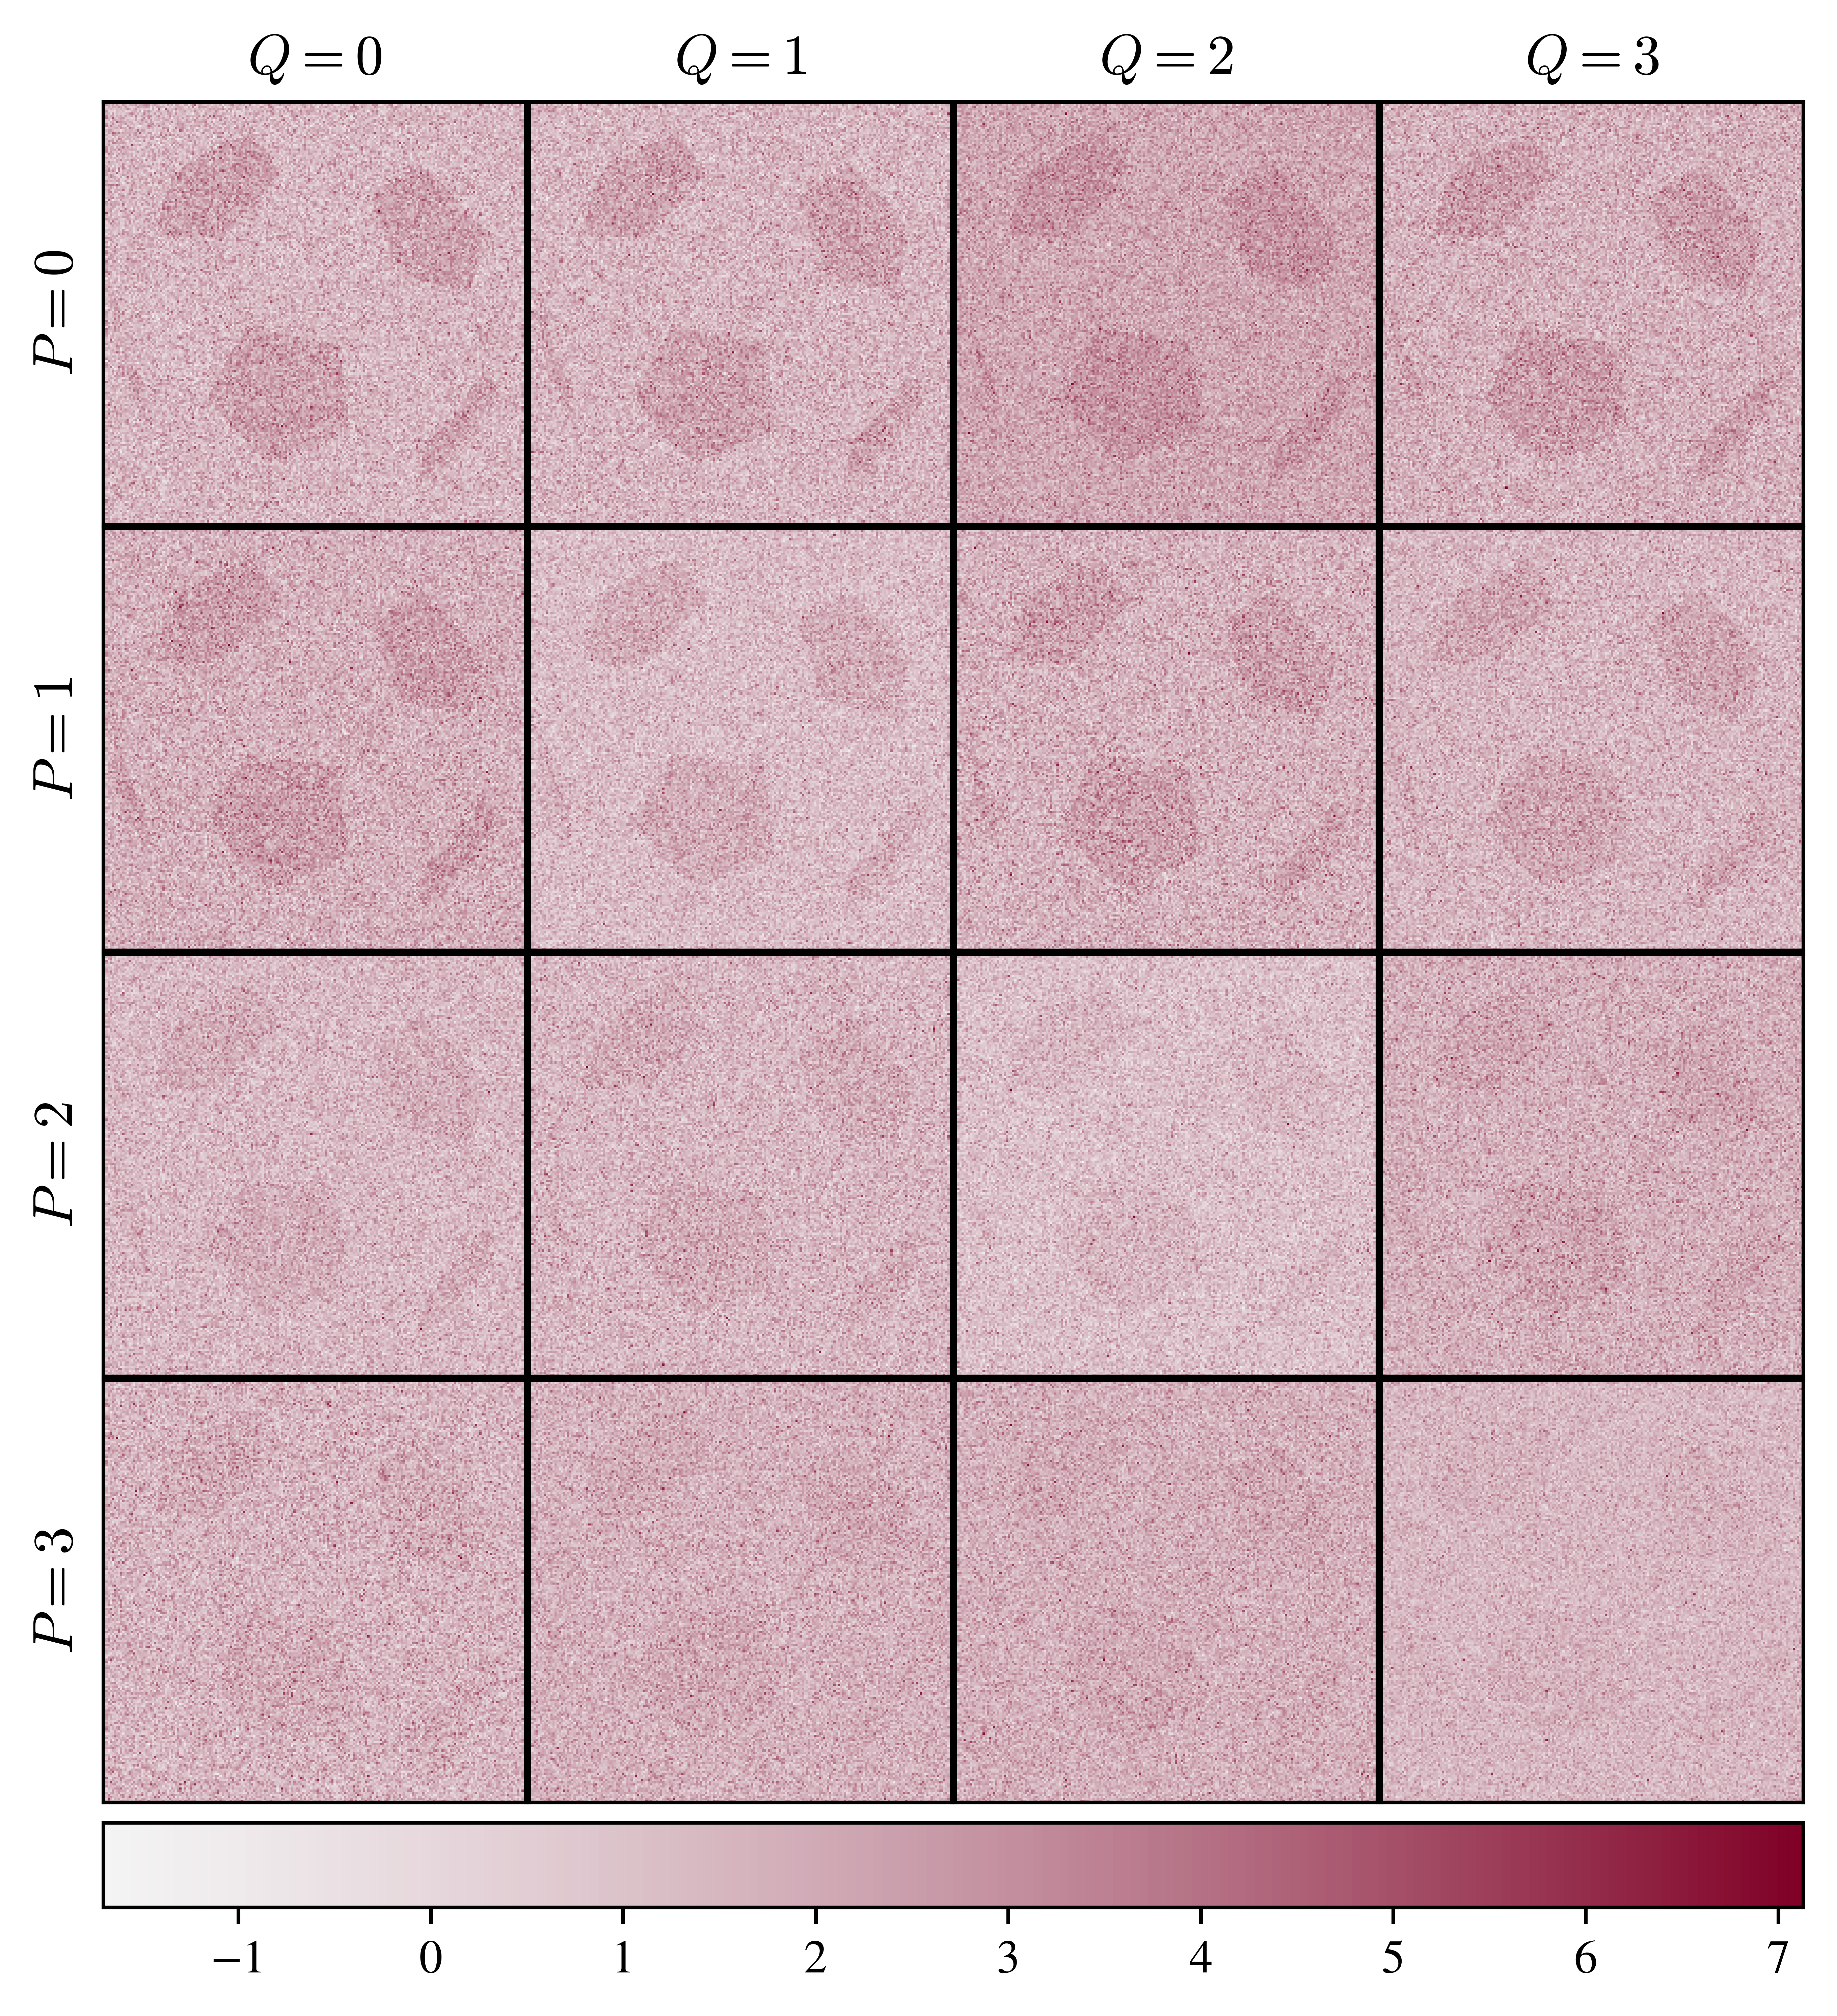
\includegraphics{images/snr2D_Spatial.png}
\caption{Spatial Distribution of the \gls{snr} Values in \gls{2d} Map}
\label{fig:snr2DSpatial}
\end{figure}

\begin{figure}[htbp!]
\centering
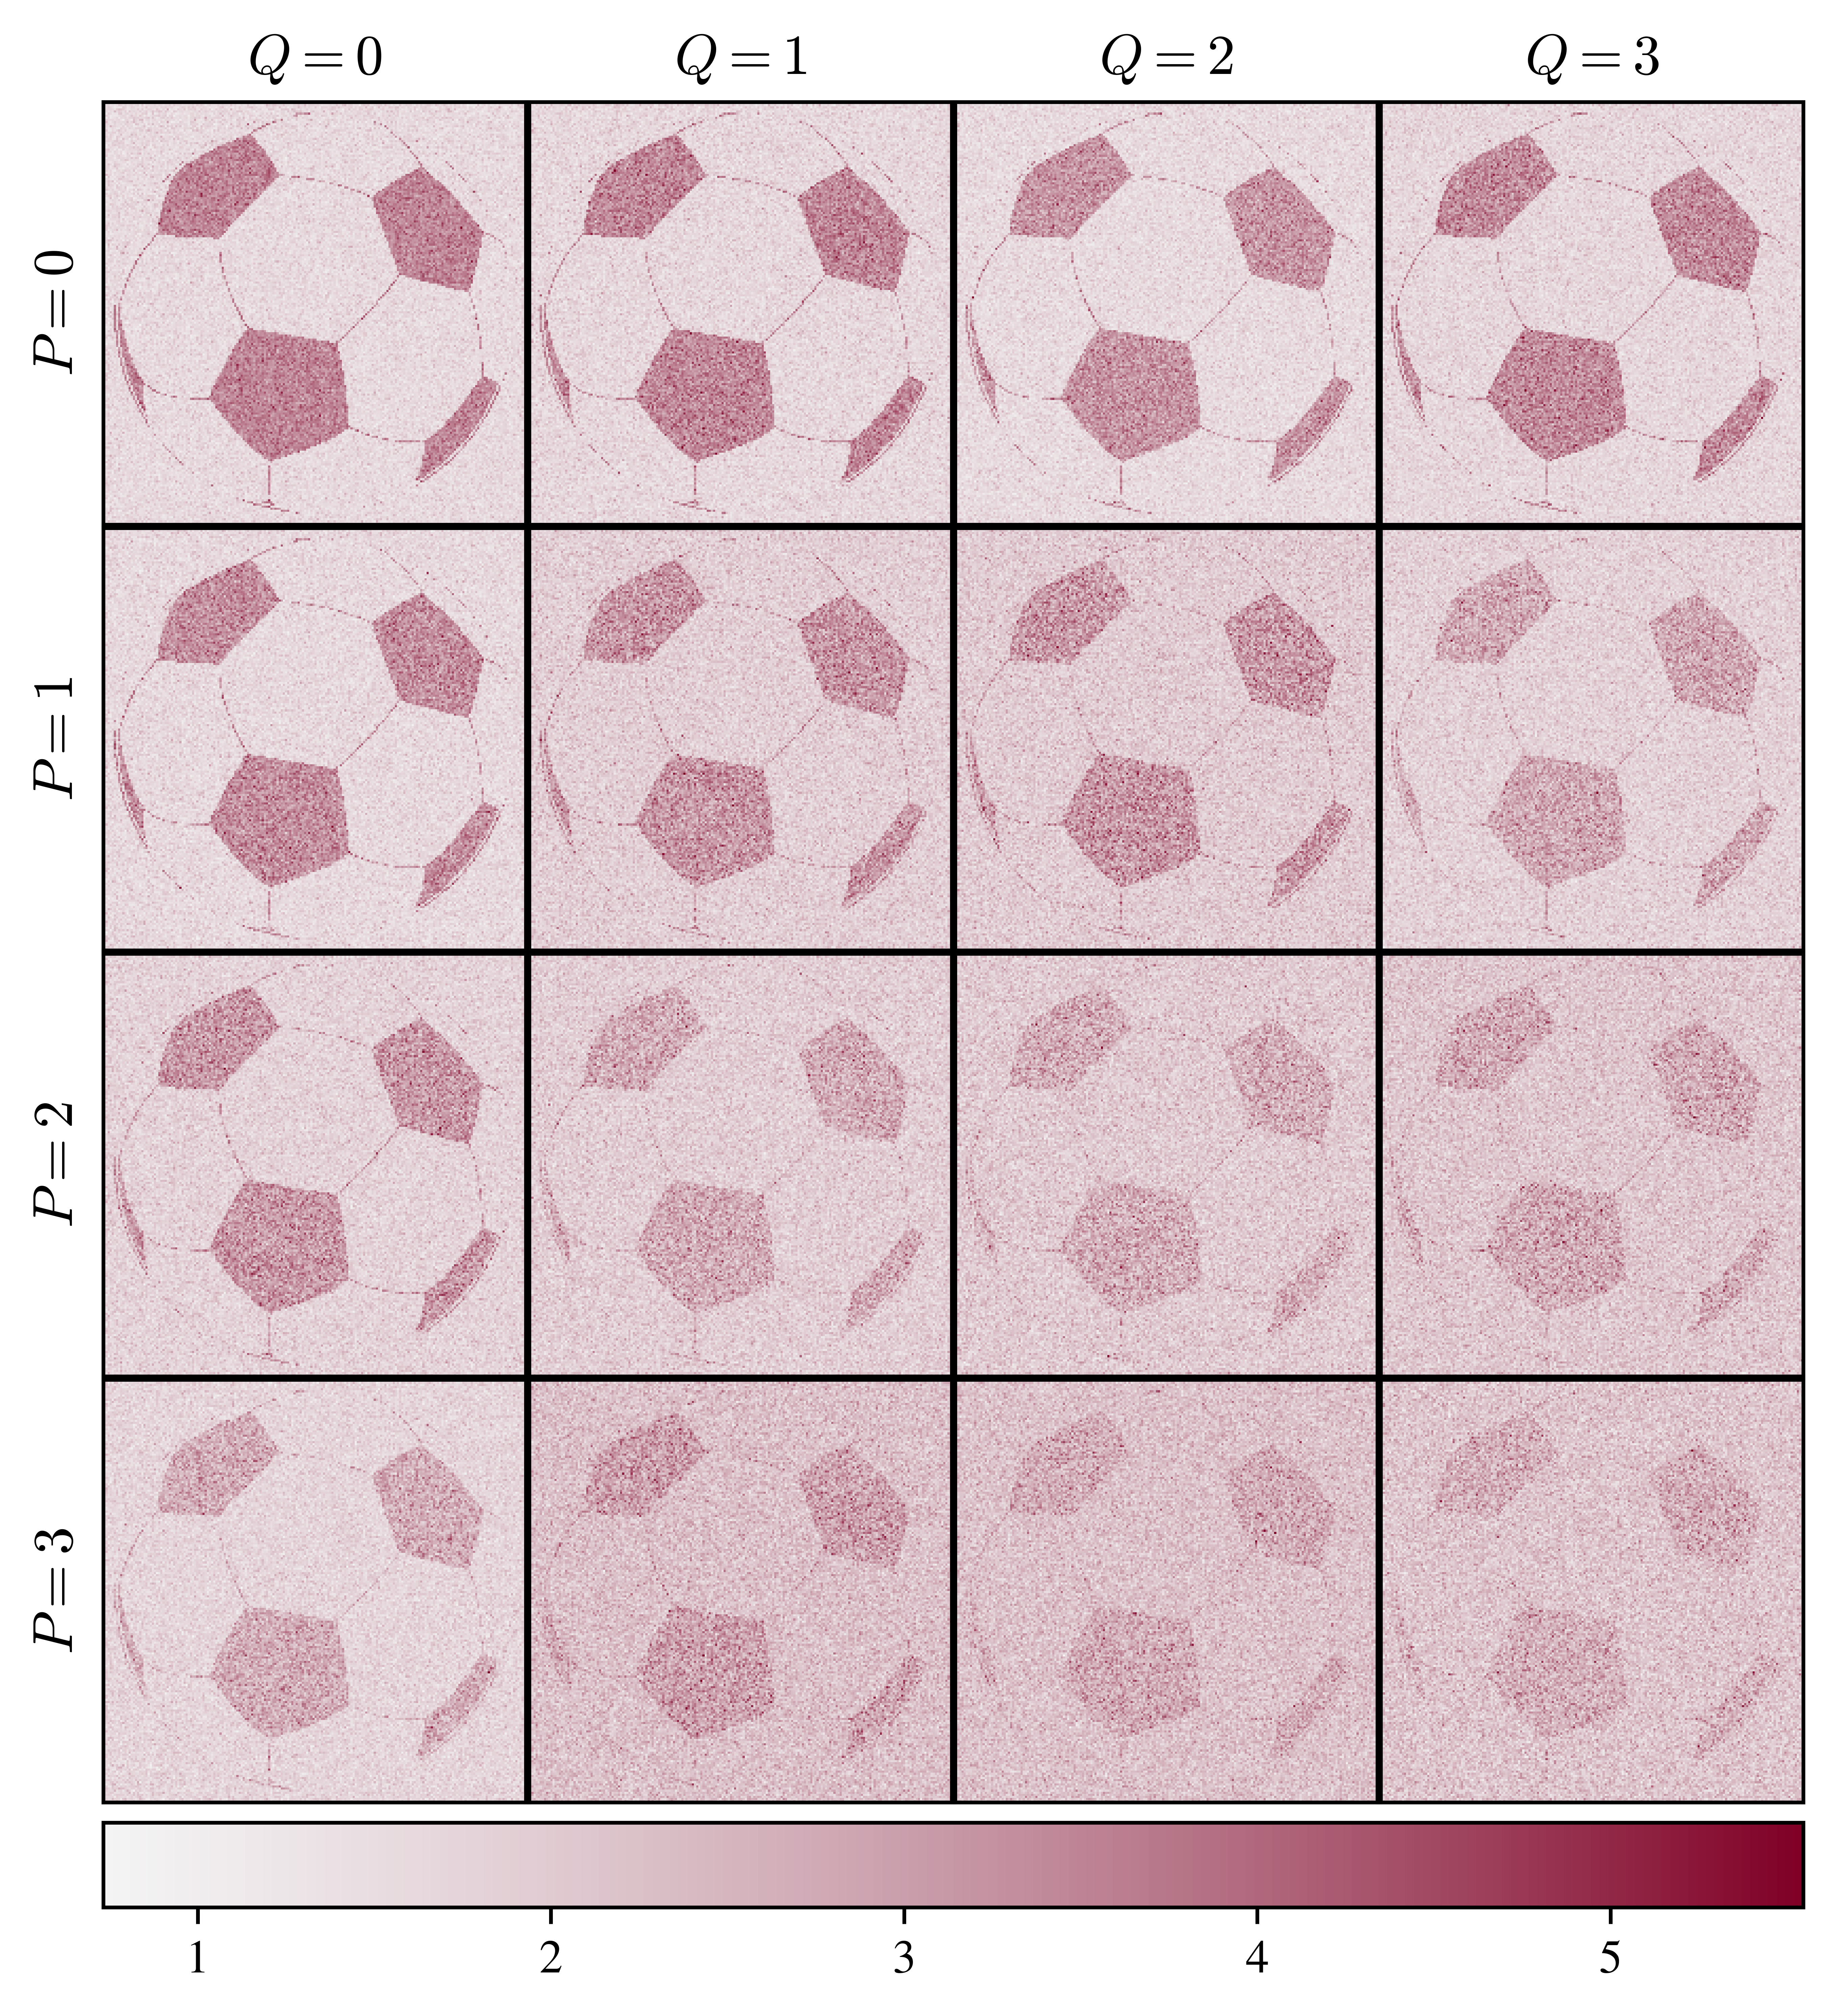
\includegraphics{images/cnr2D_Spatial.png}
\caption{Spatial Distribution of the \gls{cnr} Values in \gls{2d} Map}
\label{fig:cnr2DSpatial}
\end{figure}

\newpage

\section{Example of the Procedure}

In the following figures, examples of the results of probability and activation maps during 
the \gls{bfast} algorithm are shown for $p=0$ and $q=0$. The \gls{2d} case is seen in 
Figure \ref{fig:bfastEx2D} and the $z=20$ plane of the \gls{3d} case is seen in 
Figure \ref{fig:bfastEx3D}.

\begin{figure}[htbp!]
\centering
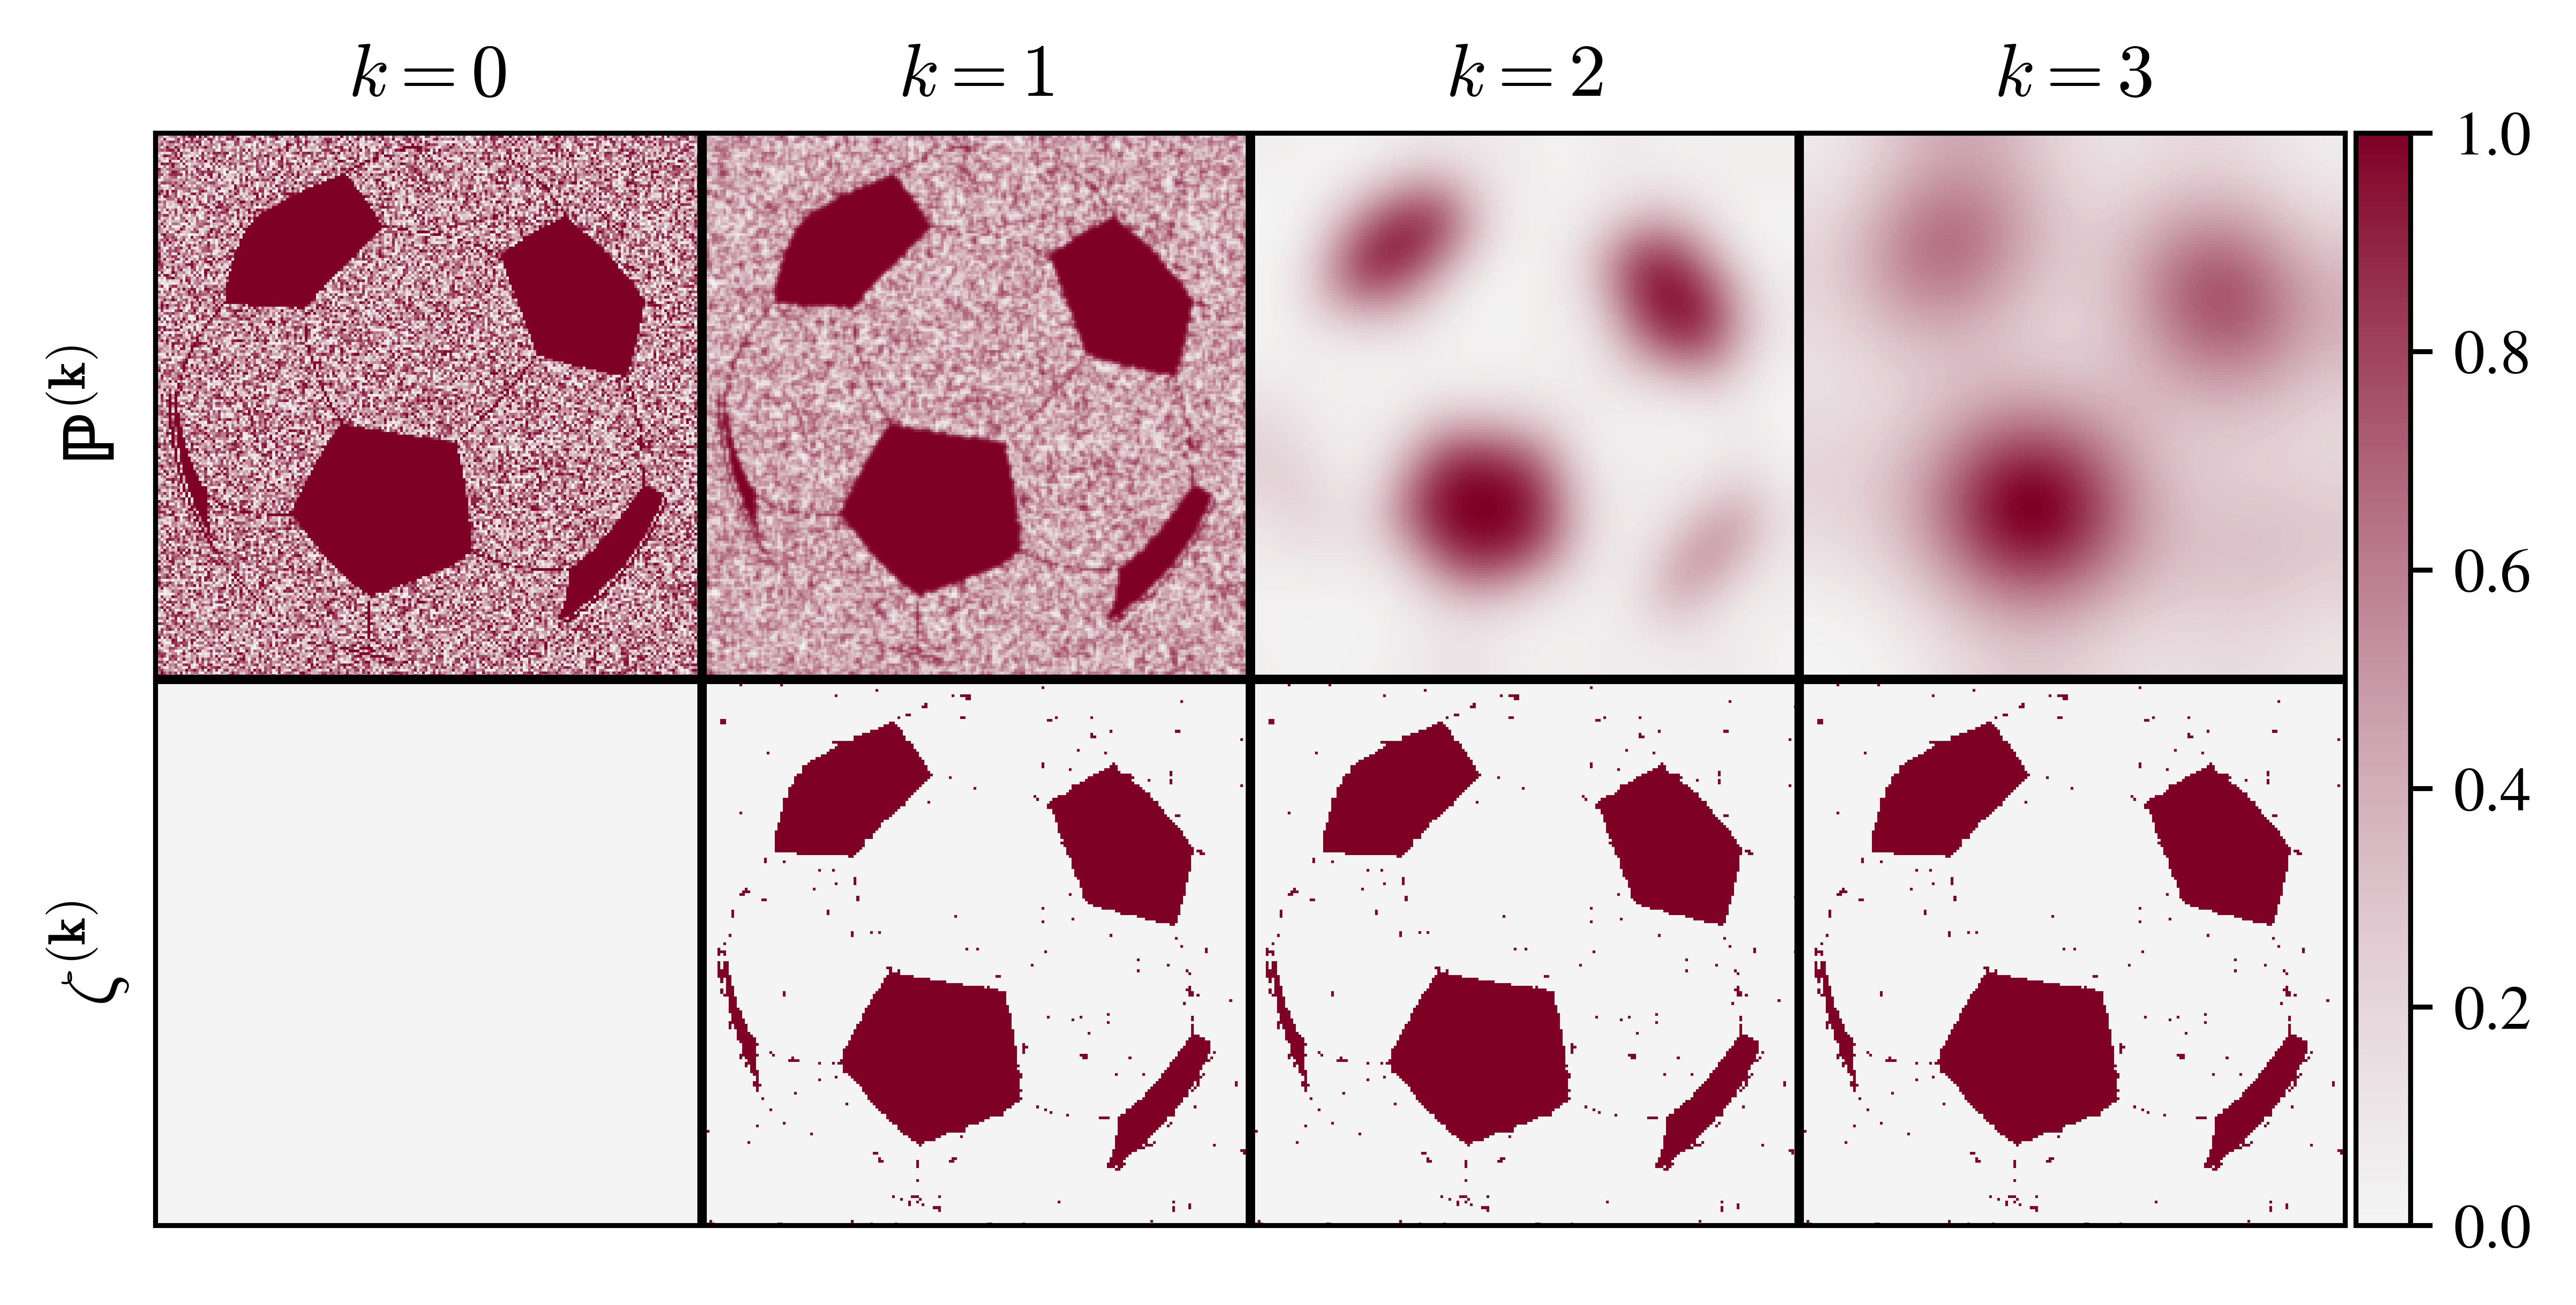
\includegraphics{images/bfastEx2D.png}
\caption{Example of Probability and Activation Maps During \gls{bfast} Algorithm for $p=0$ and $q=0$ in a \gls{2d} Map}
\label{fig:bfastEx2D}
\end{figure}

\begin{figure}[htbp!]
\centering
\includegraphics[width=0.8\textwidth]{images/plot3dSimActPr2.png}
\caption{Example of Probability and Activation Maps During \gls{bfast} Algorithm for $p=0$ and $q=0$ in the \gls{3d} Map}
\label{fig:bfastEx3D}
\end{figure}

\newpage

\section{Performance Metrics}

The performance of the \gls{bfast} algorithm was evaluated by comparing the final activated map with the true activation map using:

\begin{itemize}
\item \gls{ji}: Similarity between the two maps.
\item \gls{fpr}: Ratio of the voxels marked as activated that are not really active and the 
total number of inactive voxels.
\item \gls{poa}: Percentage of active voxels in final activation map. Recall from Table \ref{tab:aMaps} 
that expected values are $19.9375 \%$ and $3.9525 \%$ for the \gls{2d} and \gls{3d} maps, respectively.
\end{itemize}

See Tables \ref{tab:perfSum2D} and \ref{tab:perfSum3D} for the summary of these performance 
metrics in the \gls{2d} and \gls{3d} cases, respectively. Additionally, note from 
Figures \ref{fig:ji2D} and \ref{fig:ji3D} the numerical distribution of
\gls{ji} in each configuration of the simulations in the \gls{2d} and \gls{3d}
cases, respectively. As expected, the accuracy of the \gls{bfast} algorithm decreases 
as the order of the $ARMA$ model increases. However, note that the \gls{ji} in the \gls{2d} case
is around 0.9 and in the \gls{3d} case is around 0.7. These high values confirm that the \gls{bfast}
algorithm has a good performance in different noise scenarios.

\begin{table}[htbp!]
\centering
\caption{Performance Metrics Summary in \gls{2d} Case}
\begin{tabular}{ccccccc}
\hline
\textbf{p} & \textbf{q} & \textbf{\gls{snr}} & \textbf{\gls{cnr}} & \gls{ji} & \gls{fpr} & \gls{poa} \\ \hline
\multirow{4}{*}{0} & 0 & 4.0841 & 3.0344 & 0.9256 & 0.0078 & 19.663 \\
 & 1 & 3.6815 & 2.9342 & 0.8925 & 0.0180 & 20.515 \\
 & 2 & 3.5788 & 2.9035 & 0.8754 & 0.0227 & 20.858 \\
 & 3 & 3.5688 & 2.8960 & 0.8695 & 0.0244 & 20.995 \\ \hline
\multirow{4}{*}{1} & 0 & 3.5988 & 2.9042 & 0.8794 & 0.0222 & 20.870 \\
 & 1 & 2.7538 & 2.6993 & 0.8509 & 0.0299 & 21.398 \\
 & 2 & 2.5159 & 2.6191 & 0.8488 & 0.0308 & 21.475 \\
 & 3 & 2.4691 & 2.6007 & 0.8533 & 0.0292 & 21.350 \\ \hline
\multirow{4}{*}{2} & 0 & 2.9564 & 2.7050 & 0.8685 & 0.0240 & 20.908 \\
 & 1 & 2.1686 & 2.4761 & 0.8648 & 0.0267 & 21.228 \\
 & 2 & 1.8753 & 2.3861 & 0.8578 & 0.0284 & 21.333 \\
 & 3 & 1.8050 & 2.3646 & 0.8581 & 0.0283 & 21.313 \\ \hline
\multirow{4}{*}{3} & 0 & 2.5794 & 2.5607 & 0.8932 & 0.0174 & 20.445 \\
 & 1 & 1.8416 & 2.3420 & 0.8882 & 0.0185 & 20.513 \\
 & 2 & 1.5895 & 2.2576 & 0.8837 & 0.0200 & 20.638 \\
 & 3 & 1.5260 & 2.2323 & 0.8793 & 0.0213 & 20.740 \\ \hline
\end{tabular}
\label{tab:perfSum2D}
\end{table}

\begin{table}[htbp!]
\centering
\caption{Performance Metrics Summary in \gls{3d} Case}
\begin{tabular}{ccccccc}
\hline
\textbf{p} & \textbf{q} & \textbf{\gls{snr}} & \textbf{\gls{cnr}} & \gls{ji} & \gls{fpr} & \gls{poa} \\ \hline
\multirow{4}{*}{0} & 0 & 4.0430 & 2.6156 & 0.7677 & 0.0046 & 3.8075 \\
 & 1 & 3.6401 & 2.5873 & 0.7249 & 0.0068 & 3.9950 \\
 & 2 & 3.5348 & 2.5699 & 0.6796 & 0.0086 & 4.0675 \\
 & 3 & 3.5233 & 2.5660 & 0.6767 & 0.0082 & 3.9950 \\ \hline
\multirow{4}{*}{1} & 0 & 3.5553 & 2.5687 & 0.6741 & 0.0092 & 4.1500 \\
 & 1 & 2.7134 & 2.4836 & 0.6468 & 0.0108 & 4.2650 \\
 & 2 & 2.4711 & 2.4406 & 0.6410 & 0.0116 & 4.3550 \\
 & 3 & 2.4303 & 2.4320 & 0.6757 & 0.0099 & 4.2625 \\ \hline
\multirow{4}{*}{2} & 0 & 2.9143 & 2.4583 & 0.6979 & 0.0083 & 4.1125 \\
 & 1 & 2.1205 & 2.3332 & 0.6566 & 0.0108 & 4.3100 \\
 & 2 & 1.8440 & 2.2791 & 0.6909 & 0.0079 & 4.0075 \\
 & 3 & 1.7735 & 2.2584 & 0.6859 & 0.0081 & 4.0300 \\ \hline
\multirow{4}{*}{3} & 0 & 2.5407 & 2.3554 & 0.7297 & 0.0065 & 3.9650 \\
 & 1 & 1.8073 & 2.2290 & 0.7194 & 0.0067 & 3.9525 \\
 & 2 & 1.5582 & 2.1729 & 0.7167 & 0.0074 & 4.0600 \\
 & 3 & 1.5004 & 2.1515 & 0.7092 & 0.0066 & 3.8925 \\ \hline
\end{tabular}
\label{tab:perfSum3D}
\end{table}

\begin{figure}[htbp!]
\centering
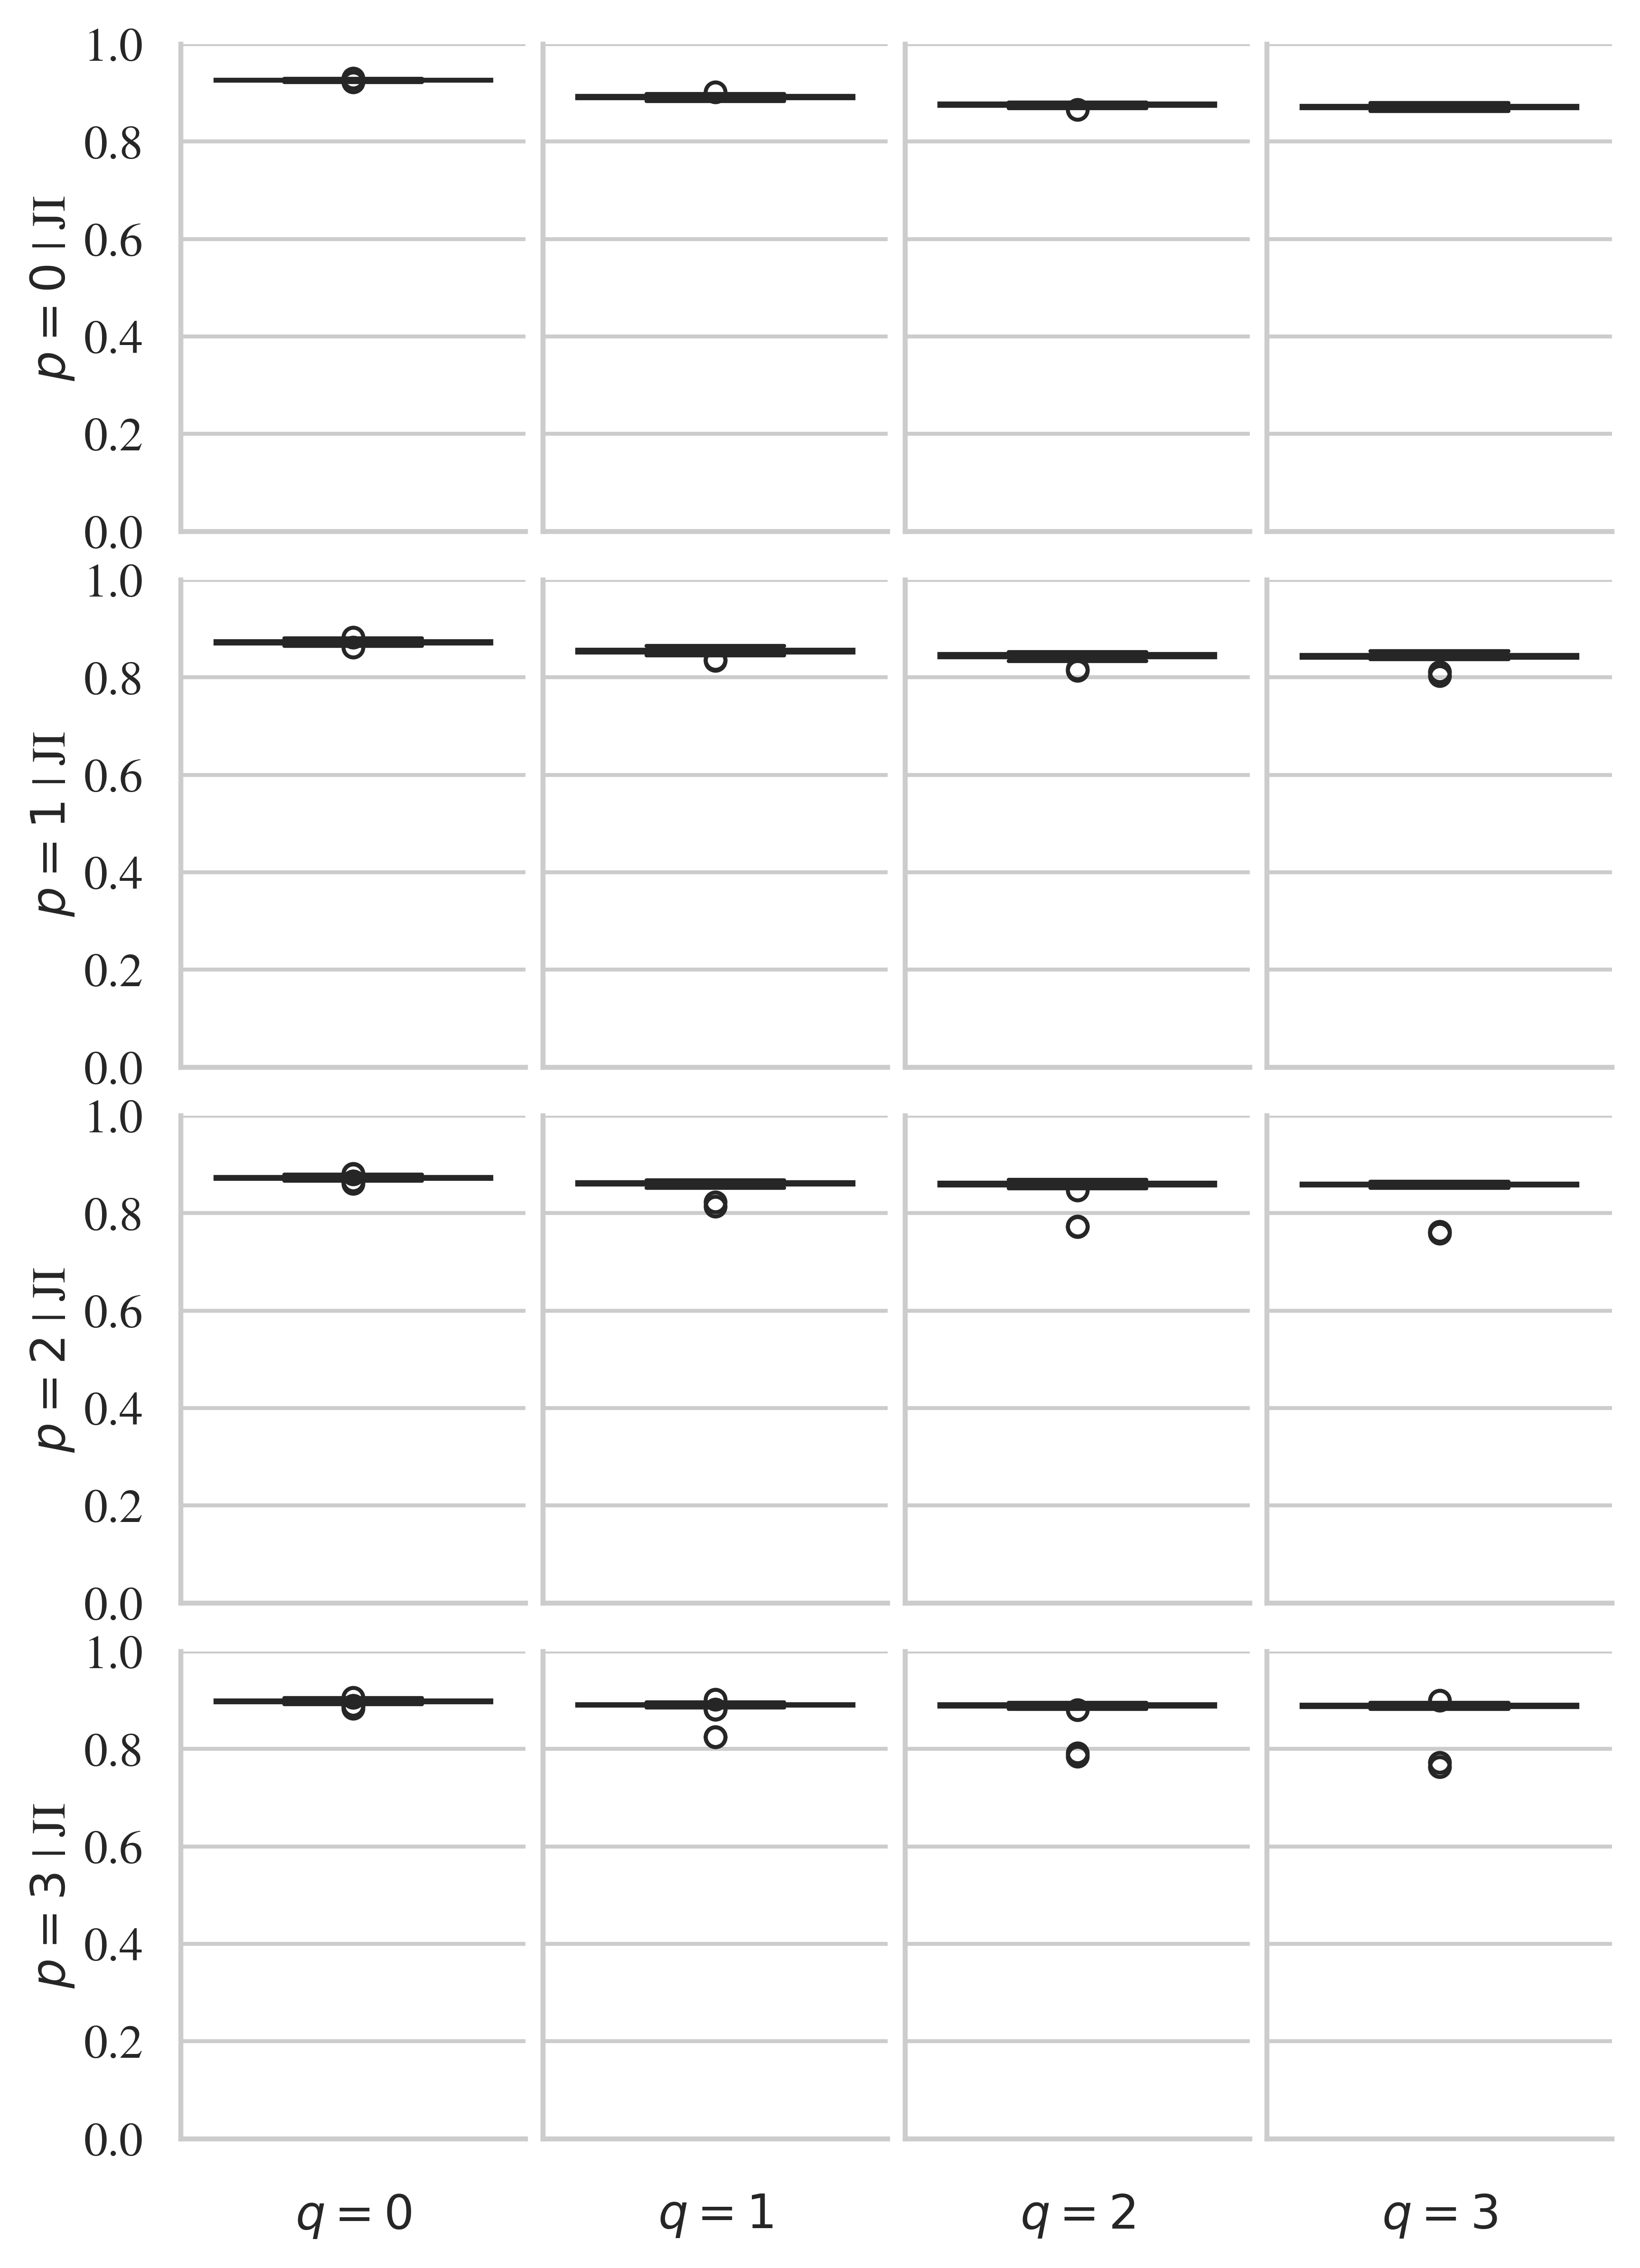
\includegraphics{images/ji2D.png}
\caption{Numerical Distribution of the \gls{ji} Values in \gls{2d} Map}
\label{fig:ji2D}
\end{figure}

\begin{figure}[htbp!]
\centering
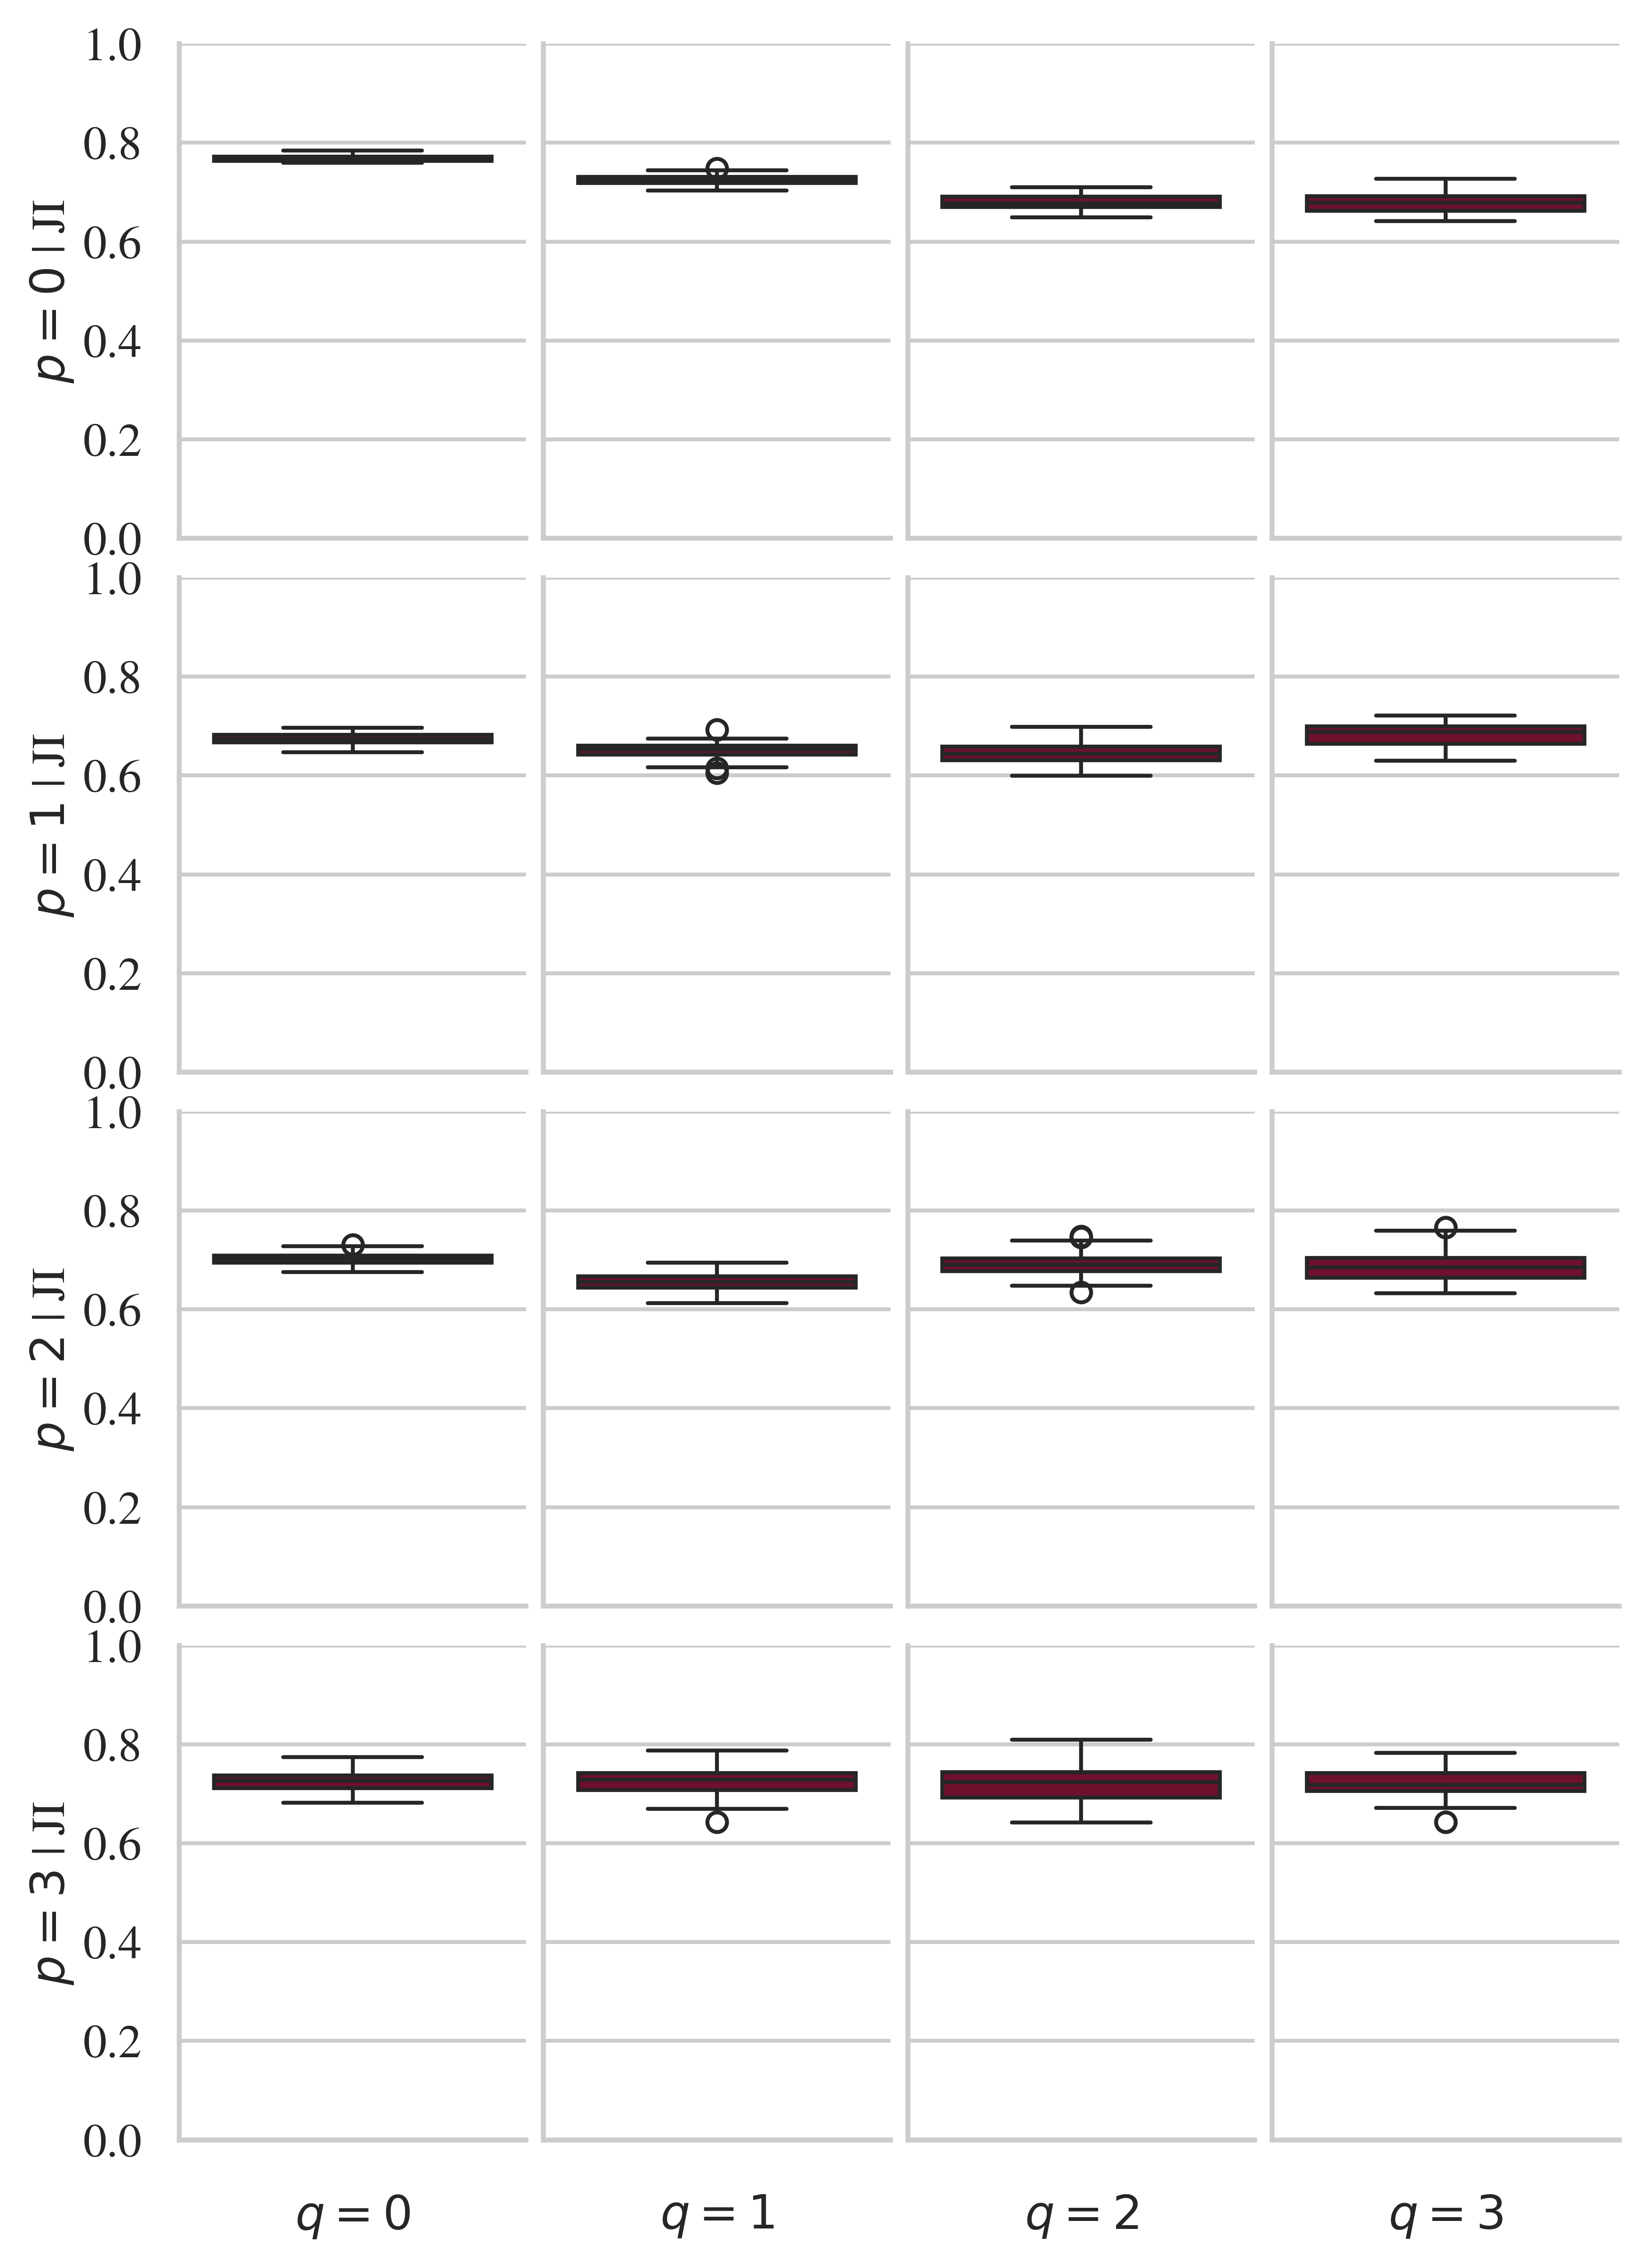
\includegraphics{images/ji3D.png}
\caption{Numerical Distribution of the \gls{ji} Values in \gls{3d} Map}
\label{fig:ji3D}
\end{figure}
\chapter{\texorpdfstring{\gls{bfast}}{BFAST} in a Real Dataset}

The \gls{bfast} Algorithm was used in the dataset of the Theory of Ming \gls{fmri} experiment 
by Moran (2012) \cite{moran2012social}. 
In this experiment, 31 participants of age around 23 and 17 participants of age around 72 were 
subject to several cognitive stimulus and data from their brain was compiled using a
gradient-echo echo-planar pulse sequence on a 3T Tim Trio MRI scanner. The machine produces data with  
dimensions $72\times72\times36$ of 2 mm isotropic voxels. It has 
recorded data from 179 timeframes taken every 2 seconds. The events log reports four types of stimulus 
which are false belief question (fbq), false belief story (fbs), false photo question (fpq), and 
false photo story (fps). In order to test and analyze the \gls{bfast} Algorithm results, only 
the data for the false belief question stimulus of the run 1 for the subject 1 was taken into 
consideration. The design matrix considered for this data is presented in Figure \ref{fig:desMatEx}.

\begin{figure}
\centering
\includegraphics[width=0.8\textwidth]{images/dMatEx.png}
\caption{Design Matrix of Run 1 of Subject 1 of Moran (2012) Experiment}
\label{fig:desMatEx}
\end{figure}

\gls{bfast} algorithm identified 1766 active voxels ($4.41\%$ \gls{poa}). In Figure
\ref{fig:realDataYZ}, the activation regions on some cuts of the brain are shown. 
This percentage of activation seems correct compared to the average percentage of activation in
\gls{fmri} experiments \cite{lazar2008statistical}. The results also suggest that the prefrontal 
cortex is active during the stimulus, this appears to be reasonable because the prefrontal cortex is 
where some part of the memory of humans is processed and this is common in this types of cognitive 
tasks \cite{amin2012brain}. Additionally, the occipital lobe also appears to be active and that is
because the stimulus are presented visually.

\begin{figure}[htbp!]
\centering
\includegraphics[width=0.9\textwidth]{images/plot3dActFinalNuevo.png}
\caption{Activation Regions in Run 1 of Subject 1 During a False Belief Question Stimulus According to \gls{bfast} Algorithm}
\label{fig:realDataYZ}
\end{figure}
%

\chapter{Results}  

\section{Section}
\noindent \lipsum[1][1-3] %WRITE HERE

\subsection{Subsection}
\noindent \lipsum[1][3-5] %WRITE HERE

\subsubsection{Subsubsection}
\noindent \blindtext %WRITE HERE

\subsection{Subsection}
\noindent \lipsum[1][2-5] %WRITE HERE

\subsubsection{Subsubsection}
\noindent \lipsum[1][1-5] %WRITE HERE

\section{Section}
\noindent \lipsum[1][5-8] %WRITE HERE

\subsection{Subsection}
\noindent \lipsum[1][9-15] %WRITE HERE



\chapter{Conclusions}

In this thesis, we've introduced a new approach for detecting brain activity 
in single subject \gls{fmri} data using adaptive smoothing and 
thresholding alongside with some Bayesian analysis. Our work has met its 
main goals, providing valuable 
insights and tools for the analysis of neuroimaging data.

We started by performing a Bayesian time-series analysis to create a 
posterior probability map for single-subject \gls{fmri} images. This bayesian 
approach handles the \gls{fmri} data in a very effective and structured manner 
such that the resulting probability maps present a reliable image 
of potential brain activations. Next, we developed an adaptive smoothing and 
thresholding algorithm called \gls{bfast} to process these probability maps and 
identify the active brain regions. By dynamically adjusting the probabilities 
given their spatial distribution, our method improves the detection of true 
activations while reducing noise. This adaptive approach ensures that the true 
active voxels are detected at each step and errors due to noise is reduced, enhancing 
the overall accuracy and reliability of the results.

We tested our algorithm extensively through various simulation scenarios. 
The results showed that our method performs well in terms of similarity 
measures, false positive rates, and the percentage of detected activations. 
These simulations demonstrated that our approach is effective, 
especially in challenging conditions with low \gls{snr} values. Finally, we applied our algorithm to a real \gls{fmri} dataset, which confirmed 
its practical utility. The real-world application showed that our method 
can detect brain activations that align with established patterns 
of brain activity. 

In summary, this thesis has developed and validated a new bayesian adaptive 
smoothing and thresholding method for detecting brain activity in single-subject 
\gls{fmri} data. Our contributions include a bayesian analysis framework, 
an adaptive processing method, and thorough testing through simulations and 
real data.

%Future Works

Modify parameters from the \gls{bfast} algorithm such as the
normalization coefficients, the computation of the threshold,
and the smoothing coefficient, among others.

Compare the results obtained by the \gls{bfast} algorithm in real life
applications with the results obtained by equivalent methods.

\appendix
\chapter*{APPENDICES}
\addcontentsline{toc}{chapter}{APPENDICES}
% Appendices are just more chapters, with different labeling (letters instead of numbers).
\chapter{Domain of Maximal Attraction Verification}
\label{ap:theoremVer}

In this section we are going to verify numerically the Theorem for the Truncated Normal Distribution using Python. For that, we first need to define the generalized normal distribution:

\begin{equation} \label{eq:Normal_PDF}
\phi (x; \mu, \sigma^2) = \frac{1}{\sigma \sqrt{2 \pi}} e^{-\frac{\left( x - \mu \right)^2}{2\sigma^2}}
\end{equation}

\begin{equation} \label{eq:Normal_CDF}
\Phi (x; \mu, \sigma^2) = \int_{-\infty} ^x \phi (t;\mu,\sigma^2) dt
\end{equation}

In Python:

Now, we define the truncated normal distribution in $(0,1)$, because we have a distribution of probabilities:

\begin{equation} \label{eq:TNormal_PDF}
\psi (x; \mu, \sigma^2,0,1) = 
\begin{cases}
0 & \text{ if } x \leq 0 \\
\frac{\phi(x;\mu, \sigma^2)}{\Phi (1; \mu, \sigma^2)-\Phi (0; \mu, \sigma^2)} & \text{ if } 0 < x < 1 \\
0 & \text{ if } x \geq 1
\end{cases}
\end{equation}

\begin{equation} \label{eq:TNormal_CDF}
\Psi (x; \mu, \sigma^2,0,1) = \int_{0} ^x \psi (t;\mu,\sigma^2,0,1) dt
\end{equation}

In Python:

Now, part $(c)$ of the theorem states that sufficient conditions for $\Psi$ to belong to $D(G_3)$, where $G_3$ is the Gumbel distribution are:

\begin{itemize}
\item If $\psi(x) >0$ and is differentiable for all $x$ in $(x_1,\epsilon_1)$ for some $x_1$, and
\begin{equation} \label{eq:partC_theorem}
\lim_{x \rightarrow \epsilon_1} \frac{d}{dx} \left[ \frac{1-\Psi(x)}{\psi(x)} \right] = 0
\end{equation}
\end{itemize}

Numerically, we take arbitrary values for $\mu$ and $\sigma$, then we substitute values for $x$ within our domain $(0,1)$ to obtain the following results.

\begin{figure}[htbp!]
\centering
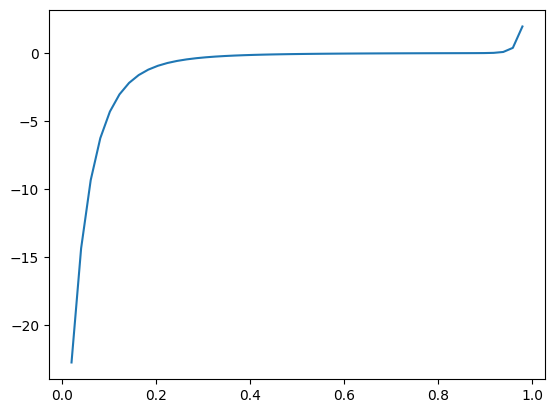
\includegraphics[width=0.7\textwidth]{images/th1052_gumbel_verify.png}
\label{fig:gumbel_verify}
\end{figure}

Note that the function inside the limit on Equation \ref{eq:partC_theorem} tends to $0$ inside the $(0,1)$ interval. Hence, Gumbel distribution can be used as a limiting distribution.
\chapter{\texorpdfstring{\gls{3d}}{3D} True Maps Generation}
\label{ap:3dMapsGen}

The procedure used to generate the \gls{3d} maps is explained below
with the following Python functions. First, Listing 
\ref{lst:createImage} presents the \textit{createImage} function,
which is the final step that creates the map, the inputs 
of this function are the dimensions of the map. This function creates a
\gls{3d} space and randomly selects some coordinates inside this space.
Now, note that this function requires the usage of the 
\textit{createActivationCluster} function, shown in 
Listing \ref{lst:createActivationCluster}. The objective of this second
function is to generate activation clusters around the randomly selected
coordinates. This clusters have a random shape within a fixed radious.
Finally, we use the functions \textit{activateLoners} and \textit{surrAct} shown 
in Listings \ref{lst:activateLoners} and \ref{lst:surrAct}, respectively. This 
functions have the task to correct the shape of the previously generated clusters
so they do not have unusual holes in them.

\begin{lstlisting}[language=Python, caption=\textit{createImage} Function, label=lst:createImage]
def createImage(dimX,dimY,dimZ):
    p = (np.random.random((dimX,dimY))>0.99).astype(int)
    base = np.zeros((dimX,dimY,dimZ))
    s = p.shape
    for i in range(s[0]):
      for j in range(s[1]):
        if p[i,j]:
          k = np.random.randint(0,dimZ)
          createActivationCluster(base,i,j,k,2*dimZ)
    return(base)
\end{lstlisting}

\begin{lstlisting}[language=Python, caption=\textit{createActivationCluster} Function, label=lst:createActivationCluster]
def createActivationCluster(array,i,j,k,size):
    r = int(np.round(np.sqrt(size*3/4/np.pi)))
    array[i,j,k] = 1
    for x in range(-r,r+1):
      for y in range(-r,r+1):
        for z in range(-r,r+1):
          if np.linalg.norm([x,y,z]) <= r:
            try:
              array[i+x,j+y,k+z] = int(np.random.randint(3)>0)
            except:
              pass
    activateLoners(array)
\end{lstlisting}

\begin{lstlisting}[language=Python, caption=\textit{activateLoners} Function, label=lst:activateLoners]
def activateLoners(array):
    s = array.shape
    for x in range(s[0]):
      for y in range(s[1]):
        for z in range(s[2]):
          if array[x,y,z] == 0:
            if surrAct(array,x,y,z):
              array[x,y,z] = 1
\end{lstlisting}

\begin{lstlisting}[language=Python, caption=\textit{surrAct} Function, label=lst:surrAct]
def surrAct(array,i,j,k):
    s = 0
    for x in [-1,1]:
      for y in [-1,1]:
        for z in [-1,1]:
          try:
            s += array[i+x,j+y,k+z]
          except:
            pass
    if s >= 4:
      return(True)
    else:
      return(False)
\end{lstlisting}
\chapter{Python Scripts}
\label{ap:pythonScripts}

\bibliography{referencias} 
%\include{backmatter}
			
\end{document}